\documentclass[11pt,a4paper]{article}
\usepackage[T1]{fontenc}
\usepackage{lmodern}
\usepackage[margin=25mm,headheight=14pt]{geometry}
\usepackage{amsmath,amssymb,amsthm,mathtools}
\usepackage{microtype,booktabs,longtable,tabularx,array}
\usepackage{graphicx,xcolor,enumitem,listings,fancyhdr}
\usepackage[hyphens]{url}
\usepackage[colorlinks=true,linkcolor=teal!60!black,citecolor=teal!60!black,urlcolor=teal!60!black]{hyperref}
\usepackage[nameinlink,noabbrev]{cleveref}
\definecolor{ink}{HTML}{17324D}
\definecolor{accent}{HTML}{167D8D}
\definecolor{shade}{HTML}{F2F5F7}
\hypersetup{pdftitle={Dual Forests and Homological Progress Certificates for Compressed Unknot Hierarchies},pdfauthor={Research contribution prepared for the ProveIt project},pdfsubject={Certified normal-cut simplification and quantitative hierarchy research}}
\newtheorem{theorem}{Theorem}[section]
\newtheorem{lemma}[theorem]{Lemma}
\newtheorem{proposition}[theorem]{Proposition}
\newtheorem{corollary}[theorem]{Corollary}
\theoremstyle{definition}
\newtheorem{definition}[theorem]{Definition}
\newtheorem{question}[theorem]{Research question}
\theoremstyle{remark}
\newtheorem{remark}[theorem]{Remark}
\newcommand{\cut}{\mathbin{\backslash\!\backslash}}
\newcommand{\Complete}{\texttt{COMPLETE}}
\newcommand{\Inconclusive}{\texttt{INCONCLUSIVE}}
\newcommand{\code}[1]{\texttt{\small #1}}
\newcolumntype{Y}{>{\raggedright\arraybackslash}X}
\newcolumntype{P}[1]{>{\raggedright\arraybackslash}p{#1}}
\setlist{itemsep=3pt,topsep=5pt}
\lstset{basicstyle=\ttfamily\footnotesize,breaklines=true,columns=fullflexible,keepspaces=true,frame=single,rulecolor=\color{black!15},backgroundcolor=\color{shade},showstringspaces=false}
\pagestyle{fancy}
\fancyhf{}
\fancyhead[L]{\small\color{ink}Compressed unknot recognition}
\fancyhead[R]{\small Research contribution \textbar\ October 2026}
\fancyfoot[C]{\thepage}
\renewcommand{\headrulewidth}{0.3pt}
\setlength{\emergencystretch}{2em}
\setlength{\parskip}{4pt}
\setlength{\parindent}{1.2em}
\setcounter{tocdepth}{1}
\hypersetup{bookmarksdepth=2}
\title{\color{ink}\LARGE\bfseries Dual Forests and Homological Progress Certificates\\[4pt]
\Large for Compressed Unknot Hierarchies}
\author{Research contribution prepared for the ProveIt project}
\date{12 October 2026\\[5pt]\small Source baseline: \texttt{8cb7d9d25ac8cb64a9d147304e3441e98e94c7a4}}

\begin{document}
\maketitle
\begin{abstract}
We develop two concrete contributions toward a compressed implementation of
Lackenby's unknot-recognition programme. First, for the authenticated bounded
core of any normal cut in the current finite-source contract, we reconstruct
the two sides of every source endpoint-gap two-handle and prove that their
dual multigraph is connected to exposed boundary. Every rooted spanning tree
therefore cancels all source three-handles, relative to the existing bundle
ports, with a trace of size independent of normal-coordinate magnitudes.
A maximum-weight tree minimizes retained additive attaching incidence. An
explicit five-tetrahedron solid torus proves a strict advantage: one forest
leaves a persistent stopping set, while the weighted forest permits a complete
geometric certificate. We also characterize successful forests by stopping-set
transversals, derive a graphic-rank obstruction, and refute a general matroid
exchange hypothesis for raw-peelable rows.

Second, we give an integer-certificate alternative for membership in the
rational image of bundle homology. Under explicitly authenticated hierarchy
hypotheses, an outside-image certificate forces a strict decrease of Lackenby's
quadratic potential, with an exact raw-cut defect formula. The algebraic
checker is implemented separately; its geometric compiler remains open.
The integrated top reduction increases certified classifications from 85 to
92 on the pinned 106-case cut corpus, preserves every prior success, and has
independent replay and explicit-cut validation. These are proved local
advances. We identify the missing global depth, branching, pattern-transport,
and encoding estimates needed for either announced quasi-polynomial bound.
\end{abstract}

\begingroup
\small
\setlength{\parskip}{0pt}
\tableofcontents
\endgroup
\clearpage
\section{Research objective, source baseline, and quantitative target}
\label{sec:context}

The immediate objective is to turn compressed normal-surface data into more
useful, independently checked geometric operations. The eventual objective
is a deterministic unknot recognizer with a proved quasi-polynomial
worst-case bound in the number of crossings of its input diagram. These
objectives are connected, but they require different theorems. A fast orbit
routine, a successful terminal handlebody test, or a polynomial-size positive
certificate does not by itself control the total number of surfaces or
hierarchy states an algorithm must inspect.

This contribution supplies a new source-relative compiler step and a
separate, exact certificate of a sufficient condition for hierarchy progress.
The first is integrated into the existing cut-classification pipeline. The
second is an algebraic research component whose future geometric interface
is specified explicitly. Their proofs, implementation, negative examples,
and experimental limits are part of one deliverable.

\subsection{The pinned state of ProveIt}

All baseline comparisons use repository revision
\begin{center}
\texttt{8cb7d9d25ac8cb64a9d147304e3441e98e94c7a4}.
\end{center}
The snapshot is from 12 October 2026. The 905 original runtime-directory
blobs were authenticated against their Git
blob identifiers. The delivered patch is relative to that revision, rather
than an unpinned moving branch. The incoming research packages in the same
snapshot were also inspected before choosing the present contribution
\cite{repo,prior-genus,prior-stopping,prior-saturated,prior-hierarchy,prior-sparse}.

The relevant existing pipeline starts from a compact, connected, orientable
finite triangulation with one torus boundary and an admissible normal
coordinate vector. It constructs the actual cut in compressed form:
a bounded complementary handle core, interval-bundle families with binary
multiplicities, and authenticated ordered interfaces. The terminal operator
then certifies a census of handlebody components when its geometric
cancellation and bundle-attachment criteria apply.

The word \Complete\ in that operator means an exact classification of the
\emph{supplied cut}: every component is certified to be a handlebody and its
genus and multiplicity are computed. It is not a complete decision procedure
for arbitrary handlebodies, and it is not a standalone knot verdict. A
nontrivial knot exterior can have a cut consisting of handlebodies. The word
\Inconclusive\ records the failure of this particular positive compiler,
not a proof that a component is a non-handlebody or that a knot is nontrivial.

The pinned terminal operator certifies 85 of the maintained 106 source cuts.
Ten unresolved inputs are rejected immediately because the source core
contains three-handles. The first theorem family below removes that entire
\emph{structural refusal}: every source three-handle can be cancelled after
the normal cut. Later positive cancellation still need not complete. On this
corpus seven of the ten inputs become certified, giving 92 successes.

\subsection{Prior results that this article uses}

The following distinctions prevent repeated work from being presented as a
new discovery.

\begin{itemize}
\item The incoming \emph{Genus Budgets and Native Interfaces} contribution
already proves completeness of the ordinary source two/three queue before
a normal cut and with the initial empty boundary pattern. Classical
two/three cancellation is also prior work. The new result concerns the
\emph{compressed complementary core after an arbitrary normal cut}, its
endpoint-gap side table, preservation of bundle ports, and independent
source replay.
\item The unsigned stopping-set characterization of positive raw one/two
cancellation, complete column peeling, and the associated unit-permanent
minor criterion are already in the incoming stopping-core work. Our new
use couples those obstructions to the set of allowable source dual forests
and realizes a strict forest-choice advantage in an actual small manifold.
\item Saturated bundle cancellation is already incorporated in the pinned
baseline. Consequently, 78 successes is an obsolete comparison point for
this patch. The appropriate baseline is 85.
\item The chain-space separation theorem used for the second component is
finite-dimensional rational linear algebra. The contribution is its exact
certificate contract, independent integer replay without trusting a
purported complete bundle-cycle basis, and its precise use with Lackenby's
equality case. We do not claim a new general linear-algebra duality theorem.
\end{itemize}

These results extend the repository's current research programme. Assertions
of priority beyond that programme would require a broader historical review;
none is needed for the geometric and algorithmic claims proved here.

\subsection{What exactly has Lackenby announced?}
\label{subsec:announcements}

The available primary sources contain two quantitative formulations. The
February 2021 talk displays a bound of the form
\[
 n^{O(\log n)}=\exp\bigl(O((\log n)^2)\bigr),
\]
and discusses logarithmic hierarchy depth. The March 2021 Oxford handout
instead displays
\[
 2^{O((\log n)^3)}=n^{O((\log n)^2)},
\]
with a corresponding squared-logarithmic depth formulation. Here $n$ is the
crossing number of the supplied diagram. Both bounds are quasi-polynomial,
but they are quantitatively different; the February bound is the stronger
target \cite{lackenby2021feb,lackenby2021mar}. The Oxford announcement also
describes an $n^{c\log n}$ bound \cite{oxford2021}.

The July 2026 preprint \emph{Incompressible surfaces, hierarchies and unknot
recognition}, already included among the project's source material, develops
the geometric hierarchy machinery \cite{lackenby2026}. Its Section 9
explicitly leaves running-time estimates outside the precision of the stated
algorithm. In particular, a quantitative iteration bound and a linear bound
in quadratic handle complexity are not themselves either 2021 asymptotic
claim. This article uses the preprint's stated theorems, while treating the
global quasi-polynomial estimate as a research target requiring additional
proofs.

\subsection{Parameters and levels of certification}

We distinguish four sizes throughout the article:
\[
\begin{aligned}
 n&=\text{diagram crossings},&
 t&=\text{source tetrahedra},\\
 L&=\text{maximum coordinate bit length},&
 W&=\sum_i x_i.
\end{aligned}
\]
The source input has size $O(t\log(t+1)+tL)$ in a direct encoding. Normal
weight $W$ may be exponential or larger relative to $t$; a compressed
operation must charge arithmetic to $L$, not loop once per normal disc.
Later chain-matrix results use their explicit ranks and entry bit lengths
as separate input parameters. There is no established identification of all
those ranks with a polynomial in $n$ along an arbitrary future hierarchy.

Three logical levels must also remain distinct. A chart-level verifier
authenticates geometric incidence from the triangulation and coordinates.
A local certificate, such as a dual forest, proves a transformation of that
authenticated geometry. A global recognition theorem must additionally
establish that the algorithm finds an adequate sequence of such operations,
terminates correctly on both answers, and spends the claimed total time.
The delivered native patch implements the first two levels for a new useful
transformation. The final sections specify the missing work at the third.

\section{Eliminating top handles after a compressed normal cut}
\label{sec:cut-dual}

The ordinary, uncut source presentation already has a complete two/three
handle reduction.  The incoming \emph{Genus Budgets and Native Interfaces}
article, Section ``The complete initial empty-pattern compiler'', states
its queue rule and proves completeness by connectivity of the source
one-skeleton.  That result, and classical handle cancellation itself, are
prior work~\cite{prior-genus}.  The extension here concerns the bounded complementary core
\emph{after an arbitrary normal cut}.  It identifies both sides of every
endpoint-gap two-handle, proves that the resulting dual graph is still
rooted-connected, preserves the authenticated interfaces with the
parallelity bundle, and makes the reduction independently replayable
without expanding normal coordinates.  In particular, the existing
\texttt{core\_has\_three\_handles} refusal is not an unavoidable obstruction
for this source family.

\subsection{The source contract and the geometric side table}

Let $\mathcal T$ be a finite triangulation of a compact connected
three-manifold $M$ with nonempty boundary.  In the implemented contract,
$M$ is orientable and has one torus boundary; the topological argument
below needs only the indicated finite-manifold and boundary hypotheses.
Vertex links must be discs or spheres, and reversed self-identifications
of an edge are excluded.  Let $S$ be an embedded normal surface, possibly
disconnected, one-sided, or empty, given by admissible nonnegative integer
normal coordinates $x$.  By cutting along $S$ we mean removing the
interior of a small regular neighbourhood and taking the resulting compact
manifold with rounded corners.

Use the authenticated source parallelity decomposition
\[
  M\mathbin{\backslash\!\backslash}S=K\cup_A B.
\]
Here $B$ is the union of the specified interval bundles, $K$ is the bounded
complementary handle core, and $A=K\cap B$ is its port subsurface.  This
notation does not assume that $B$ is globally a product.  The source
construction puts all its core-facing ports in boundary charts of the
zero- and one-handles of $K$; the two-handles considered below are the
\emph{endpoint gaps} at source edges.  The endpoint gaps are distinct from
the interior edge gaps that belong to the parallelity bundle.

For a source edge $e$, choose its globally consistent orientation and let
$v_-(e),v_+(e)$ be its two endpoint occurrences.  Their global vertex
identifiers may coincide.  Put
\[
  w(e)=|S\cap e|.
\]
Let $V_{\mathrm{int}}$ be the set of interior source vertices and use a
formal symbol $\ast$ for exposed boundary.  Define
\[
 \rho(v)=
 \begin{cases}
   v,&v\in V_{\mathrm{int}},\\
   \ast,&v\in\partial M.
 \end{cases}
\]
Each $v\in V_{\mathrm{int}}$ supplies one source three-handle, irrespective
of the normal coordinates.  A source boundary edge supplies no core
two-handle.  An interior source edge supplies one endpoint-gap two-handle
when $w(e)=0$ and two when $w(e)>0$.

\begin{lemma}[The exact dual side table]
\label{lem:cut-dual-sides}
The two belt-disc sides of the source core two-handles have the following
owners:
\[
\begin{array}{c|c|c}
 \text{normal edge weight}&\text{source gap rank}&\text{ordered side owners}\\
 \hline
 w(e)=0&0&(\rho(v_-(e)),\rho(v_+(e)))\\
 w(e)>0&0&(\rho(v_-(e)),\ast)\\
 w(e)>0&w(e)&(\ast,\rho(v_+(e))).
\end{array}
\]
An occurrence of $\ast$ means an exposed face on the original boundary
or on the boundary created by cutting $S$.  Repeated interior owners are
retained with their multiplicity: $(v,v)$ means two intersections with
the attaching sphere of the same three-handle, not one.
\end{lemma}

\begin{proof}
Give an edge neighbourhood its source product chart
$D^2\times e$.  The normal surface meets the edge in $w(e)$ distinct
points.  Its complementary intervals are the gaps between successive
normal points and the two endpoint gaps.  A core two-handle is
$D^2\times J$, where $J$ is an endpoint gap; its belt sphere consists of
the two points at the centres of $D^2\times\partial J$.

If $w(e)=0$, the single gap runs between the two source vertices.  A
finite interior vertex contributes its vertex-link three-ball, while a
boundary vertex contributes an exposed boundary chart.  This gives the
first row.  If $w(e)>0$, the initial gap runs from the initial vertex to
the first normal point, and the final gap runs from the last normal point
to the final vertex.  Their normal-point sides are exposed after cutting.
The intervening gaps, if present, lie in $B$ and are not endpoint-gap
core handles.  This gives the second and third rows.

The argument is local at the edge.  It does not require a coorientation
of $S$: the two sides of each individual intersection point have local
product neighbourhoods even when the whole surface is one-sided.
Likewise, if the endpoint occurrences represent the same global vertex,
they are still distinct ends of the edge chart and give distinct belt
points.  This proves the multiplicity assertion.
\end{proof}

There is a direct formula for reconstructing this table from the existing
records.  A zero-handle flag in a two-handle attaching cycle gives a local
source edge $(t,[a,b])$, with $a<b$.  The signed source edge equivalence
relation gives a bit $\epsilon(t,a,b)$.  Its ordered endpoint flags are
$(t,a),(t,b)$ when $\epsilon=0$ and $(t,b),(t,a)$ when $\epsilon=1$.
The three-handle vertex-link triangles assign an interior owner to each
such vertex flag; unassigned flags must be authenticated boundary vertices.
The edge weight can also be checked locally:
\begin{equation}
 w(e)=x_{t,a}+x_{t,b}
       +\sum_{j=0}^{2}x_{t,4+j}-x_{t,4+q(a,b)},
 \label{eq:cut-dual-local-weight}
\end{equation}
where $q(a,b)$ is the quadrilateral type that misses the edge $[a,b]$.
Every term actually contributing to the right side is nonnegative.
Normal matching makes this value the same around the entire source edge.
An independent checker can therefore inspect \emph{every} source
zero-handle flag in the cycle and require the same oriented side pair;
it need not trust a producer's chosen representative.

\subsection{A universal rooted forest in the cut core}

Define a multigraph $G_x$ with vertex set $V_{\mathrm{int}}\cup\{\ast\}$
and one edge for each source endpoint-gap two-handle, joining the owners
in Lemma~\ref{lem:cut-dual-sides}.  Both parallel edges and loops are
retained.  Several boundary components of the cut manifold may be
represented by the same formal root.  This is an indexing device: the
algorithm never glues these boundary components together.

\begin{lemma}[Rooted connectivity survives normal cutting]
\label{lem:cut-dual-connected}
Every vertex of $G_x$ is connected to $\ast$.
\end{lemma}

\begin{proof}
The source one-skeleton is connected.  Fix an interior vertex $v$ and
choose an edge path from $v$ to a source boundary vertex, stopping at the
first boundary vertex encountered.  Every edge before this final endpoint
is an interior edge, since a boundary edge has both endpoints on the
boundary.

If all edges on the path have weight zero, the first row of
Lemma~\ref{lem:cut-dual-sides} turns it into a path in $G_x$ ending at
$\ast$.  Otherwise, follow the initial weight-zero part of the path.
At the first positive-weight edge, the endpoint gap incident to the
current vertex joins that vertex directly to $\ast$.  Either case gives
the required rooted path.  No upper bound on a nonzero edge weight has
been used.
\end{proof}

\begin{lemma}[Relative top-handle cancellation]
\label{lem:cut-dual-relative}
Suppose an endpoint-gap two-handle has exactly one side on a surviving
three-handle and its other side is exposed.  This pair can be cancelled
geometrically.  The resulting presentation retains the original zero-
and one-handle records and the original attaching curves of every
unselected two-handle.  The induced homeomorphism can be chosen to fix
the port subsurface $A$.
\end{lemma}

\begin{proof}
The belt sphere of a two-handle $D^2\times I$ is the two-point set
$\{0\}\times\partial I$.  By hypothesis, the attaching sphere of the
chosen three-handle meets precisely one of those points and does so once
in its source product chart.  It does not meet the other point, which
lies on exposed boundary.  This is the geometric two/three cancellation
condition, with actual belt intersections rather than a signed cellular
coefficient.

The elementary cancellation pushes the three-ball through this single
two-handle to the exposed side.  Equivalently, in the reversed handle
picture it absorbs a zero-handle and its single connecting one-handle
into a boundary collar.  There is no other surviving three-handle using
the selected two-handle, so no other top attaching sphere needs to slide
over this pair.  All remaining two-handles retain their attaching maps
to the zero/one stage.

The source port rectangles come from interior bundle gaps of ranks $1,\ldots,w-1$, whereas selected core gaps have ranks $0$ or $w$. Source vertex three-ball neighbourhoods contain no bundle. Thus the source port rectangles lie in the zero/one boundary charts and are
disjoint from the attaching regions and belt faces of the endpoint-gap
two-handle and from the vertex-link attaching sphere.  Shrinking the
source collars slightly gives a cancellation neighbourhood disjoint
from $A$.  The cancellation is the identity outside that neighbourhood,
so its induced pair-homeomorphism fixes $A$.  This assertion concerns the
presentation and the specified port subsurface.  It does not assert a
pointwise identification of the entire old zero/one submanifold with the
entire new one.
\end{proof}

\begin{theorem}[Complete cut-relative elimination of three-handles]
\label{thm:cut-dual-complete}
For every authenticated source normal cut above and every spanning tree
$D$ of $G_x$, there is a geometric two/three cancellation sequence that
deletes exactly the two-handles indexed by $D$ and all source three-handles.
The resulting core $K_D$ satisfies
\[
  (K_D,A)\cong(K,A),\qquad
  K_D\cup_A B\cong M\mathbin{\backslash\!\backslash}S.
\]
Its zero/one records and all unselected two-handle attaching cycles are
unchanged.  In particular, it has the same Euler characteristic as $K$.
\end{theorem}

\begin{proof}
Root $D$ at $\ast$ and process its other vertices in any order in which
parents precede children.  For a vertex $v$, select the two-handle of its
parent edge.  Its $v$ side still meets the attaching sphere of the
three-handle $v$ exactly once.  The other side is either originally
exposed or belongs to a parent three-handle already absorbed into the
exposed boundary.  It is therefore exposed at this stage.  Apply
Lemma~\ref{lem:cut-dual-relative}.

Induction deletes one distinct two-handle and one distinct three-handle
per nonroot vertex.  No selected edge is a loop.  A spanning tree has
exactly $|V_{\mathrm{int}}|$ edges, so all three-handles are deleted.
Each step is relative to $A$, hence so is the composite homeomorphism.
Extend this homeomorphism by the identity on $B$ to recover the whole
cut manifold.  Each cancellation removes one handle contributing $+1$
and one contributing $-1$ to Euler characteristic, which proves the
last assertion.
\end{proof}

There is also a direct embedded-ball interpretation of the proof.
Remove the formal root from the selected tree.  Every remaining tree
component has exactly one selected half-edge leading to exposed boundary;
two such half-edges would make a cycle through the root.  Its source
vertex three-balls, joined by the selected endpoint-gap tubes, form a
regular neighbourhood of a tree and hence a three-ball.  This ball meets
the boundary of $K$ in the single exposed cap disc.  Its remaining
frontier is also a disc, so removing it reverses the elementary attachment
of a ball along a boundary disc.  The source port charts miss these
selected handles.  Thus the ball removal is relative to $A$.  This
description does not replace the port contract by a homology computation:
the tree and its product charts give an actual embedded ball.

The theorem covers an empty normal surface, a one-sided normal surface,
and arbitrary binary multiplicities.  It assumes the validity of the
authenticated source charts; arbitrary three-handle summaries or group
presentations are not substitutes.  It does not assert that the resulting
core is a handlebody.  Raw one/two cancellation, bundle attachment tests,
closed bundle bases, and later hierarchy conditions remain separate.

\begin{corollary}[Compatibility with bundle consumers]
\label{cor:cut-dual-consumers}
Any subsequent construction whose geometric inputs are the original
zero/one core charts, the unselected two-handle cycles, and the
authenticated port subsurface can instead use $K_D$.  In particular,
source disk-bundle absorption and the existing relative bundle attachment
constructions are valid after the top reduction.  An absorbed additional
two-handle is not an eligible edge of $G_x$ and cannot be selected by the
top-cancellation certificate.
\end{corollary}

\begin{proof}
The required charts and attaching subsurface are preserved by
Theorem~\ref{thm:cut-dual-complete}.  Thus the construction attaches exactly
the same geometric pieces along the same port data.  Added two-handles
arise from the specified later attachments, rather than from source edge
endpoint gaps; they have no source vertex-link side authentication and
are kept outside the eligible graph.
\end{proof}

An arbitrary later boundary pattern need not be supported on $A$.  It may
cross an exposed face of a selected endpoint-gap two-handle.  Transporting
such a pattern is not supplied by the preceding theorem.  The relative
scope is precisely the authenticated bundle ports and any marks supported
there.

\subsection{Support dependence and small reusable certificates}

\begin{proposition}[The dual graph depends only on zero support]
\label{prop:cut-dual-support}
For a fixed source triangulation, $G_x$ depends only on the set
\[
  Z(x)=\{e:w_x(e)=0\}.
\]
Here an edge address is $(e,0)$ when its weight is zero and $(e,-)$ or
$(e,+)$ for its initial or final gap when its weight is positive.  If
$Z(x)=Z(y)$, these addresses identify $G_x$ with $G_y$.  Every rooted
forest trace for one is therefore a valid trace for the other after
independent source authentication.  In particular, this applies to
$y=mx$ for every positive integer $m$.
\end{proposition}

\begin{proof}
The interior vertices, boundary vertices, and oriented endpoint owners
are fixed by the source.  The side table has only the dichotomy $w=0$
or $w>0$; no positive magnitude appears in any owner.  Hence the stated
addresses give identical multigraphs.  A rooted trace only records those
edges and their endpoint owners, so the same root-before-child argument
replays it.  Finally, $w_{mx}(e)=m w_x(e)$ has the same zero set for $m>0$.
\end{proof}

The normal source coordinates and any other source certificate still need
to be checked for each input.  The proposition reuses the combinatorial
top trace, not the truth of source authenticity.  An edge-zero bit vector
of length $O(t)$ is a sufficient cache key together with the source
triangulation identifier for a graph-only choice such as breadth-first
search.  A maximum-weight strategy may depend on finer data through its
row costs: an already selected trace still replays at the same zero
support, but need not remain cost-optimal there.  Positive scalar
multiplication preserves the full bounded-core incidence combinatorics
and the fixed primal forest, so the raw-incidence costs, as well as a
deterministically tied maximum-weight choice, are also unchanged under
$x\mapsto mx$ with $m>0$.  Indeed, core zero-handles are selected by the
vanishing or positivity of triangle and quadrilateral counts, core
one-handles by the vanishing or positivity of their normal face-arc
counts, and endpoint-gap incidences by homogeneous comparisons of the
corresponding partial sums.  Multiplication by $m>0$ preserves all these
decisions.  It changes the numerical source-chamber and endpoint-rank
addresses, but not the finite handle identifiers or their incidence
cycles.  The spanning-forest choices and their literal row costs follow.

A simple certificate lists the source side pair of every endpoint-gap
two-handle, the ordered pairs
\[
  (\text{three-handle identifier},\text{two-handle identifier}),
\]
and the surviving source two-handle identifiers.  An independent checker
reconstructs the side table, checks every selected handle is live, and
requires exactly one surviving interior side, with its multiplicity
equal to one.  It then removes that three-handle and two-handle.  At the
end it requires that no three-handle survives and that the supplied
survivor list is exact.  A source side that belonged to an earlier removed
three-handle is then exposed; a loop with two live occurrences fails the
singleton test.  Survivors can be densely renumbered for a downstream
checker, while the certificate retains the original source identifier
map.  Other records, in particular all zero/one identifiers and ports,
retain their original indices.

\begin{proposition}[Combinatorial and bit costs]
\label{prop:cut-dual-cost}
Let $t$ be the number of source tetrahedra and let $L$ bound the bit length
of the normal coordinates.  Given authenticated source incidence and
coordinate data, dual graph construction, a breadth-first spanning tree,
and trace replay require $O(t)$ combinatorial incidence operations.
The added trace and side table contain $O(t\log(t+1))$ bits, independent
of normal weight magnitudes.  Recomputing the local weights by
\eqref{eq:cut-dual-local-weight} adds $O(tL)$ elementary bit work.
Independent source reconstruction and validation are additional costs.
\end{proposition}

\begin{proof}
There are at most $4t$ source vertex flags, at most $6t$ local edge
occurrences, and at most two core endpoint gaps per global interior edge.
The vertex-link flag lists have total length $4t$.  Every source edge-link
wedge appears in at most two endpoint-gap cycles, so the total number of
two-handle zero/one flag occurrences is $O(t)$.  Building the side table,
adjacency lists and rooted tree, and scanning a supplied trace therefore
use $O(t)$ incidence operations.  There is one move per interior vertex.
All identifiers and owner labels are bounded by $O(t)$, proving the bit
size bound.  A local edge weight is a sum of a bounded number of
$L$-bit coordinates, and the finite chart scan has $O(t)$ such operations.
This proves the bit-work bound.  It does not identify the cost of the
existing source-preparation routine with this already-prepared graph cost.
\end{proof}

\subsection{Choosing the top forest optimally for retained work}

A rooted breadth-first tree guarantees completion of the top phase, but
different trees delete different two-handle rows.  This gives an exact
and inexpensive optimization that does not presume that incidence size
determines downstream recognizability.

\begin{proposition}[Spanning trees are exactly the complete deletion sets]
\label{prop:cut-dual-tree-sets}
For the source-side cancellation rule used here, the sets of two-handles
deleted by complete top-cancellation traces are exactly the spanning
trees of $G_x$.
\end{proposition}

\begin{proof}
One direction is Theorem~\ref{thm:cut-dual-complete}.  Conversely, direct
each selected edge from the three-handle removed at that move to its
other endpoint.  That endpoint is $\ast$ or a vertex removed earlier.
Following directed edges strictly decreases deletion time until it
reaches $\ast$.  Thus there is no directed or undirected selected cycle,
and every nonroot vertex has a selected path to $\ast$.  There are exactly
$|V_{\mathrm{int}}|$ selected edges.  They form a spanning tree.
\end{proof}

\begin{theorem}[Minimum retained additive incidence]
\label{thm:cut-dual-weighted}
Assign a nonnegative cost $c_h$ to each source two-handle $h$, and keep
all costs fixed during the top reduction.  A maximum-weight spanning
tree of $G_x$, with edge weight $c_h$, minimizes
\[
  \sum_{h\notin D}c_h
\]
among every complete pure top-cancellation trace.  Examples include the
total number of raw attaching occurrences or the number of distinct
nonzero incidences in a row after a fixed zero/one forest contraction.
The tree can be computed using $O(t\log(t+1))$ graph comparison operations.
\end{theorem}

\begin{proof}
Unselected two-handle rows do not change, so retained cost equals
$\sum_h c_h-\sum_{h\in D}c_h$.  Proposition~\ref{prop:cut-dual-tree-sets}
says exactly which deletion sets are allowed.  Maximizing the second
sum is the maximum-weight spanning-tree problem on a multigraph with
$O(t)$ edges.  Sorting the edges and applying the usual greedy forest
algorithm proves the complexity statement.  Loops cannot be selected;
parallel edges are treated as distinct edges.
\end{proof}

This optimum concerns an additive retained-work objective.  It does not
assert that the same tree maximizes the number of later cancellations,
produces the smallest final certificate, or finds a handlebody whenever
one exists.  Those are different optimization or recognition questions.

\subsection{Combining a dual forest with exact raw cancellation}

Fix a zero/one spanning forest and a source-authenticated nonnegative
raw incidence matrix $N=(n_{rh})$.  Its rows include every source
two-handle and may include additional geometrically authenticated
two-handles from later bundle constructions; these additional rows are
not eligible dual edges.  Its columns are the remaining one-handles.
A nonempty row set $R$ is a stopping set if
\[
  \sum_{r\in R} n_{rh}\ne 1\quad\text{for every column }h.
\]
Because the entries are nonnegative integers, these sums are zero or at
least two.  This is the established unsigned stopping condition, not
an algebraic rank or exponent-sum test.

For a rooted tree $D$, let $N\setminus D$ denote deletion of its eligible
source rows.  A raw positive pivot at $(r,h)$ requires $n_{rh}=1$, deletes
that row and column, and updates the surviving entries by
\[
 n'_{ij}=n_{ij}+n_{ih}n_{rj}.
\]
The prior complete raw-cancellation theorem~\cite{prior-stopping,prior-saturated} says that this operation can
remove all rows exactly when no nonempty stopping set exists.  Equivalently,
the unit-column peeling algorithm then removes all rows.  This prior
theorem supplies the following cut-relative consequence.

\begin{theorem}[Tree transversal criterion]
\label{thm:cut-dual-stopping}
For a fixed authenticated matrix and zero/one forest, the following
conditions are equivalent:
\begin{enumerate}
 \item Some complete source two/three forest is followed by a complete
       sequence of positive raw one/two cancellations.
 \item Some spanning tree $D$ of $G_x$ satisfies
       $\operatorname{Stop}(N\setminus D)=\varnothing$.
 \item Some spanning tree $D$ of $G_x$ meets every nonempty stopping
       set of $N$, where meeting means sharing an eligible source row.
\end{enumerate}
\end{theorem}

\begin{proof}
The possible top deletion sets are exactly the spanning trees by
Proposition~\ref{prop:cut-dual-tree-sets}.  Their effect on raw incidence
is literal row deletion.  Applying the prior raw theorem proves the
equivalence of the first two conditions.  A row set of $N\setminus D$
is a stopping set precisely when it is a stopping set of $N$ disjoint
from $D$: its entries and columns have not changed.  Therefore no such
set remains exactly when $D$ meets every original nonempty stopping set.
\end{proof}

\subsection{A native five-tetrahedron example with strict coverage gain}
\label{subsec:cut-dual-native-example}

The included fixture
\texttt{fast/core\_dual\_fixtures.py}, function
\texttt{interior\_loop\_torus()}, gives a small exact example in which
forest selection changes the existence of \emph{any} complete positive
raw continuation.  This is stronger than observing different outcomes
from two greedy one/two producers.

Here are its complete face identifications.  Tetrahedra and local vertices
are numbered from zero.  A permutation word $p_0p_1p_2p_3$ means that
source vertex $i$ maps to target vertex $p_i$.  The reverse gluing is the
inverse permutation.  The two unpaired faces are $(0,3)$ and $(1,2)$.
\[
\begin{array}{c|c|c}
 \text{one-handle}&\text{paired faces}&\text{vertex permutation}\\
 \hline
 0&(0,0)\leftrightarrow(4,1)&1230\\
 1&(0,1)\leftrightarrow(2,0)&1023\\
 2&(0,2)\leftrightarrow(1,3)&0132\\
 3&(1,0)\leftrightarrow(2,3)&3201\\
 4&(1,1)\leftrightarrow(3,0)&1023\\
 5&(2,1)\leftrightarrow(4,3)&0321\\
 6&(2,2)\leftrightarrow(3,3)&0132\\
 7&(3,1)\leftrightarrow(4,2)&0213\\
 8&(3,2)\leftrightarrow(4,0)&1302
\end{array}
\]
All nine gluing permutations are odd, so the displayed tetrahedron
orientations agree.  The source equivalence relations have two global
vertices and eight global edges.  Three edges lie in the boundary; the
remaining five are interior.  The boundary consists of two triangles
with one vertex and three edges and is a connected torus.  The finite
vertex-link data are
\[
\begin{array}{c|c|c|c|c}
 \text{source vertex}&\text{link vertices}&\text{link triangles}
       &\text{unpaired link sides}&\chi(\text{link})\\
 \hline
 0\ \text{(boundary)}&10&12&6&1\\
 3\ \text{(interior)}&6&8&0&2.
\end{array}
\]
The same face equivalence check verifies that edge links are intervals
or circles and that there is no reversed edge identification.  Thus the
vertex links are respectively a disc and a sphere; these checks certify
the finite-manifold input contract independently of any historical
fixture-generation method.

Use the zero normal coordinate vector.  There is no parallelity bundle
and the cut is the source manifold itself.  The source core has handle
counts $(5,9,5,1)$, and its canonical zero/one forest is
$T=\{0,1,2,4\}$.  In source two-handle order, the complete unsigned
one-handle passage lists and the dual side owners are
\[
\begin{array}{c|c|c|c}
 r&\text{source edge identifier}&\text{ordered passage list}
     &\text{dual side owners}\\
 \hline
 0&2 &(2,4,6,1)&(\ast,v)\\
 1&4 &(2,3,5,0)&(\ast,v)\\
 2&5 &(1,5,8,7,0)&(\ast,v)\\
 3&11&(4,7,8,6,3)&(v,\ast)\\
 4&14&(6,7,5)&(v,v).
\end{array}
\]
The vertex $v$ denotes the single three-handle.  The last dual edge is
a genuine loop with two incidences at $v$ and is ineligible for its
cancellation.  In columns $(3,5,6,7,8)$, contraction of $T$ leaves
\begin{equation}
 N=\begin{pmatrix}
  0&0&1&0&0\\
  1&1&0&0&0\\
  0&1&0&1&1\\
  1&0&1&1&1\\
  0&1&1&1&0
 \end{pmatrix}.
 \label{eq:cut-dual-native-matrix}
\end{equation}
These lists can be reconstructed simply by walking the five interior
source edge links in the face table.  The delivered independent source
checker performs that reconstruction before either top-forest replay or
raw incidence replay.

\begin{proposition}[A strict source-realized difference between forests]
\label{prop:cut-dual-native-strict}
For the source in \eqref{eq:cut-dual-native-matrix}, the canonical
breadth-first top forest leaves a matrix that admits no full positive
raw cancellation.  The maximum retained-work saving forest leaves a
matrix that does admit a complete no-fill cancellation, proving that
the source manifold is a solid torus.  Their retained raw occurrence
counts are respectively twelve and nine.
\end{proposition}

\begin{proof}
The breadth-first producer encounters the edge of row zero first and
deletes that two-handle with $v$.  The four remaining rows have column
totals
\[
  (2,3,2,3,2).
\]
Their entire row set is therefore a stopping set.  Stopping persistence
excludes every complete sequence of positive raw pivots, including
sequences that introduce fill.  This failure is not tied to the later
producer's pivot order.

The five raw row costs are $(1,2,3,4,3)$.  Eligible edges are rows zero
through three; row four is a loop.  A maximum-weight rooted tree
therefore uniquely chooses row three, with cost four.  Delete it with
the three-handle.  The surviving rows have the following unit-column
peeling sequence, written in the original source row and one-handle
labels:
\[
  (1,3),\quad(2,8),\quad(4,5),\quad(0,6).
\]
At each step the named column has total exactly one among the remaining
rows.  Hence every cancellation is geometric and introduces no fill.
After contraction of the four zero/one forest edges, the four one/two
cancellations leave one zero-handle, one one-handle, and no two- or
three-handles.  The result is a genus-one handlebody.  Since the normal
surface was empty, this is a direct geometric certificate that the
source manifold itself is a solid torus, requiring neither an
irreducibility assumption nor an external recognition oracle.

The initial raw occurrence total is thirteen.  Deleting a row of cost
one leaves twelve, while deleting the row of cost four leaves nine.
\end{proof}

The example establishes a strict useful gain for the weighted producer.
It does not show that this cost objective always finds a successful tree
whenever one exists.  Its complete source contract, small face table,
integer passage lists, and positive certificate make it reproducible
without the tool that was originally used to discover the fixture.

\subsection{Forest-independent obstructions and finite search}

\begin{corollary}[Graphic-rank obstruction for every top forest]
\label{cor:cut-dual-rank-obstruction}
Let $R_1,\ldots,R_k$ be pairwise disjoint nonempty stopping sets of $N$.
Let $U$ be the set of eligible source dual edges whose row labels belong
to $\bigcup_iR_i$.  If
\[
  r_{G_x}(U)<k,
\]
where $r_{G_x}(U)$ is the graphic-matroid rank of $U$, then no top forest
followed by positive raw cancellation can remove all rows.  In
particular, a stopping set consisting only of ineligible rows and dual
loops is such an obstruction.
\end{corollary}

\begin{proof}
A successful spanning tree must meet every $R_i$ by
Theorem~\ref{thm:cut-dual-stopping}.  Since the $R_i$ are disjoint, these
meetings require at least $k$ distinct edges of $D\cap U$.  But a subset
of a spanning tree is a forest, so
$|D\cap U|\le r_{G_x}(U)$.  This contradicts the strict inequality.
If all eligible edges of one stopping set are loops, its rank is zero.
\end{proof}

This obstruction has a short independently checkable form: list the
disjoint row sets, check their unsigned stopping sums from the source
matrix, and compute
\[
 r_{G_x}(U)=|V(G_x)|-c(V(G_x),U),
\]
including isolated vertices in the component count.  This is an
obstruction to the stated compiler family, not a certificate that the
core is not a ball or that the knot is nontrivial.

\begin{proposition}[Raw-peelable row sets need not form a matroid]
\label{prop:cut-dual-nonmatroid}
For a fixed nonnegative integral incidence matrix, let an independent
row set mean one whose induced row submatrix admits complete raw
cancellation.  These sets form a hereditary independence system, but
in general do not satisfy matroid augmentation.  A counterexample of
minimum possible row and column dimensions is
\[
 N=\begin{pmatrix}
  1&2\\
  1&1\\
  1&0
 \end{pmatrix},
 \qquad\text{with rows }a,b,c.
\]
\end{proposition}

\begin{proof}
Every row subset of a matrix with no nonempty stopping set also has no
nonempty stopping set.  The established raw theorem therefore proves
heredity.

Set $I=\{a\}$ and $J=\{b,c\}$.  The set $I$ is independent by its unit
entry in the first column.  The set $J$ is independent: its second column
has total one and removes $b$, after which the first column removes $c$.
Thus $|I|=1<2=|J|$.  However, the column totals on $I\cup\{b\}$ are
$(2,3)$, and the totals on $I\cup\{c\}$ are $(2,2)$.  Each is a nonempty
stopping set.  Neither element of $J\setminus I$ can augment $I$.

Any hereditary independence system on at most two elements is a matroid,
so three rows are necessary.  With a single column, a nonempty row set
is raw-peelable exactly when it consists of one row with entry one.
The other rows are loops of the independence system.  This is a rank-one
uniform matroid on the unit rows, together with loops, so two columns
are necessary.  The displayed matrix attains both lower bounds.
\end{proof}

This is a statement about the general unsigned incidence model; it is
not an assertion that this smallest matrix is the full incidence of a
particular source cut.  It rules out an automatic appeal to matroid
intersection for the tree-transversal condition.  Any additional
exchange property for a narrower family of source triangulations would
need a separate geometric theorem.  In particular, the additive optimum
of Theorem~\ref{thm:cut-dual-weighted} should not be advertised as an
optimum for downstream complete cancellation.

The failure is not caused solely by doubled individual incidences.
For the Boolean rows
\[
 a=(1,0,0),\quad b=(1,1,0),\quad
 c=(0,1,1),\quad d=(1,1,1),
\]
take $I=\{c,d\}$ and $J=\{a,b,c\}$.  The set $I$ peels $d$ in column
one and then $c$.  The set $J$ peels $c,b,a$ in columns three, two, one.
But the totals on $I\cup\{a\}$ are $(2,2,2)$, and those on
$I\cup\{b\}$ are $(2,3,2)$.  Thus Boolean incidence already violates
augmentation.  As before, this is a matrix statement, without an
additional claim that these rows form a particular source handle core.

\begin{proposition}[A finite complete forest search]
\label{prop:cut-dual-search}
Let $q=|V_{\mathrm{int}}|$ and $m=|E(G_x)|$.  Enumerating all $q$-element
edge subsets, retaining the spanning trees, and applying complete
unit-column peeling to $N\setminus D$ decides the equivalent conditions
of Theorem~\ref{thm:cut-dual-stopping}.  Its time is bounded by
\[
  \binom{m}{q}\operatorname{poly}(t,L,|N|)
  \le m^q\operatorname{poly}(t,L,|N|).
\]
Here $|N|$ denotes the encoded raw matrix size.  For $q=O(\log t)$ and
polynomial encoded matrix size this is quasipolynomial in $t$, apart
from the displayed polynomial dependence on coordinate bit length.
\end{proposition}

\begin{proof}
Every complete top trace deletes one of the enumerated trees.  The
independent geometric theorem permits every such tree, and exact
peeling decides full positive cancellation of its row complement.
Thus all candidates in the restricted family are considered.  The
number of candidates and the polynomial tests give the stated bound.
\end{proof}

In general $q=O(t)$, so this is an exponential worst-case search, not a
quasipolynomial unknot-recognition algorithm.  Even exhaustive success or
failure concerns a fixed source chart system, a fixed zero/one forest,
and the positive raw model.  Changes of disk system, intersection-reducing
slides, new normal cuts and arbitrary boundary-pattern transport are
outside the search.  The most useful initial implementation is therefore
the guaranteed polynomial top phase, optionally with the exact additive
tree objective, followed by the existing independently certified consumers.

\subsection{A proposed alternating optimization of the two forests}
\label{sec:paired-forests}

The implemented weighted dual-tree choice optimizes the retained literal
attaching-curve work after fixing the primal forest. There is a symmetric,
currently unimplemented optimization of the primal forest. The following
statement concerns two finite graphs and an incidence matrix; its proof
requires no additional claim about transporting boundary markings.

Let $G_{01}$ be a finite multigraph with edge set $\mathcal H$, and let
$G_{23}$ be a connected finite multigraph with distinguished root and edge
set $\mathcal R$. Loops are allowed in both graphs but cannot lie in a
forest. Let $N=(n_{rh})_{r\in\mathcal R,h\in\mathcal H}$ have nonnegative
integer entries. In the intended source application, $n_{rh}$ is the
number of literal passages of source two-handle $r$ through source
one-handle $h$. Let $T$ span every connected component of $G_{01}$ and let
$D$ be a spanning tree of $G_{23}$. Define
\[
 C(T,D)=\sum_{r\notin D}\sum_{h\notin T}n_{rh},
 \qquad M=\sum_{r,h}n_{rh}.
\]
Thus $C$ counts retained source passages after deleting the selected
source two-handles and ignoring the primal-tree one-handles. It uses raw
occurrences, without cancellation of inverse letters or any prediction of
later handle slides.

\begin{proposition}[Alternating exact forest responses]
\label{prop:paired-forests}
For fixed $T$, a maximum-weight spanning tree of $G_{23}$ with edge
weights
\[
 w_T(r)=\sum_{h\notin T}n_{rh}
\]
minimizes $C(T,D)$. For fixed $D$, a maximum-weight spanning forest of
$G_{01}$, spanning each of its components, with edge weights
\[
 v_D(h)=\sum_{r\notin D}n_{rh}
\]
minimizes $C(T,D)$ over $T$.

Starting from any feasible pair, alternate these two exact responses,
accepting a changed forest only when it strictly decreases $C$. Stop after
a complete sweep in which neither response gives a strict decrease. There
are at most $C(T_0,D_0)\le M$ accepted updates. At termination, changing
either forest alone cannot lower $C$.

Suppose the graphs have total combinatorial size $O(t)$ and the matrix is
provided as literal occurrence lists of total length $M$. Then this
procedure uses
\[
 O\bigl((M+1)(M+t\log(t+2))\bigr)
\]
word operations and $O(M+t)$ working storage. In particular, for source
incidence of size $M=O(t)$, the bound is $O(t^2\log(t+2))$ after source
construction and authentication.
\end{proposition}

\begin{proof}
For fixed $T$,
\[
 C(T,D)=\sum_{r\in\mathcal R}w_T(r)-\sum_{r\in D}w_T(r).
\]
The first term is constant, proving the dual assertion. For fixed $D$,
\[
 C(T,D)=\sum_{h\in\mathcal H}v_D(h)-\sum_{h\in T}v_D(h),
\]
which proves the primal assertion component by component. These formulas
include all loop weights in the constant terms; a loop is never silently
treated as a cancellable forest edge.

The objective is a nonnegative integer, so every accepted update lowers it
by at least one. Every nonterminal full sweep contains an accepted update.
There are consequently at most $M+1$ sweeps, including the final sweep.
If an optimal response has the current objective value, retaining the
current forest is essential to the specified stopping rule: zero-gain
changes are not performed. Thus, in the final unchanged sweep, both
current forests individually attain their conditional minimum.

One pass through the occurrence lists computes the required weights.
Sorting weighted graph edges and running the usual maximum-spanning-forest
algorithm costs $O(t\log(t+2))$ word operations per response. There are at
most two responses per sweep. All weights lie between zero and $M$, so
$O(\log(M+t+2))$-bit words suffice for weights and identifiers. This proves
the complexity and storage bounds.
\end{proof}

Conditional optimality can be strictly weaker than joint optimality even
for two-edge graphs. Give each graph two vertices joined by two parallel
edges and take
\[
 N=\begin{pmatrix}1&2\\2&0\end{pmatrix}.
\]
Deleting row two and column two leaves cost one. Changing either deletion
alone raises the cost to two, so both responses retain this pair. Deleting
row one and column one together instead leaves cost zero. This is an
abstract incidence example, without a claimed geometric realization.

This is a proposal for a producer heuristic, not a modification of the
runtime delivered here. A final chosen dual tree would still require the
independent source-side replay, and a chosen primal forest would still
need to be recorded in the applicable downstream certificate. The graph
objective does not establish transport of an arbitrary boundary pattern
through primal contractions. Nor does conditional optimality prove global
optimality over pairs, existence of a complete raw cancellation schedule,
or completeness of the recognition algorithm. The strict-update bound is
polynomial for the stated literal source representation; for an arbitrary
matrix of huge binary-encoded multiplicities, a bound proportional to the
numerical value $M$ would instead be pseudo-polynomial.

\section{Relative bundle quotients and certificates of strict progress}
\label{sec:quotient-progress}

Lackenby's equality criterion for quadratic handle complexity gives an
algebraic way to certify that a proposed surface makes strict progress.
The useful object is the part of relative second homology that is
represented inside the interior parallelity bundle. A surface whose class
survives after quotienting out that subspace cannot be one of the
homologically bundle-supported surfaces allowed by the equality case.
We make this observation quantitative and give a complete exact
certificate system for its algebraic premise.

The geometric implication below is a corollary of
\cite[Proposition~5.9]{lackenby2026}. The linear alternative is an
application of finite-dimensional duality. The contribution here is their
explicit combination with a small, independently replayable certificate
contract, including the conditions under which the algebraic result can
be promoted to a statement about the geometric algorithm.

\subsection{The pair map and the geometric hypotheses}

Let $M$ be a compact connected oriented PL $3$-manifold with boundary
pattern $P$, and let $\mathcal H$ be an admissible handle structure in the
sense of \cite[Definition~5.3]{lackenby2026}. Let $\mathcal B$ be its
\emph{actual interior parallelity bundle}, as defined in
\cite[Definition~5.6]{lackenby2026}, with the embedding in $M$ inherited
from those handles. Throughout this section use the conservative pair
\[
 A=\mathcal B\cap\partial M,\qquad
 j:(\mathcal B,A)\longrightarrow(M,\partial M).
\]
This is an inclusion of pairs, so it induces a well-defined map on
relative homology. Define
\begin{equation}
 \label{eq:quotient-bundle-image}
 V_{\mathcal B}
 =\operatorname{im}\!\left(
 H_2(\mathcal B,A;\mathbb Q)
 \xrightarrow{\,j_*\,} H_2(M,\partial M;\mathbb Q)
 \right).
\end{equation}
All chain complexes used to compute this map must come from compatible
cellular or simplicial models of the \emph{embedded} pair. An abstract
isomorphism between homology groups does not specify this image.

\begin{remark}[Horizontal boundary is an additional embedding assertion]
\label{rem:quotient-horizontal}
One can instead use $A_h=\partial_h\mathcal B$ if its actual inclusion in
$\partial M$ has been established. For the interior parallelity handles,
having no $3$-handles is a sufficient condition: the horizontal faces are
disjoint from other $0$-, $1$-, and $2$-handles and hence lie in the
manifold boundary. A general handle structure may have $3$-handles, and
horizontal faces may meet them. Thus a map
$H_2(\mathcal B,\partial_h\mathcal B)\to H_2(M,\partial M)$ must not be
formed solely from an abstract description of the bundle.
The choice $A=\mathcal B\cap\partial M$ always defines the pair map needed
here. When $A_h\subseteq A$, its image contains the image obtained from
$(\mathcal B,A_h)$, so it can make the obstruction weaker but does not
invalidate the sufficient implication. Twisted $I$-bundles are allowed.
\end{remark}

For a $0$-handle $H$, write $I(H)$ for its integer index from
\cite[Definition~5.1]{lackenby2026}. The quadratic complexity is
\[
 c_q(\mathcal H)=\sum_{H\in\mathcal H^0}
                  \bigl(\max\{I(H),0\}\bigr)^2.
\]
The subscript $q$ denotes quadratic complexity. Later the certificate
file also has a field named \texttt{q}; we denote that positive integer
by $\nu$ in the mathematics to distinguish the two uses.

\begin{theorem}[The quotient obstruction forces a positive even raw defect]
\label{thm:quotient-strict-progress}
Let $\mathcal H$, $M$, $P$, $\mathcal B$, and $A$ be as above. Let $S$ be
a compact connected oriented surface properly embedded in $M$ and normal
with respect to $\mathcal H$. Suppose
\[
 [S]\notin V_{\mathcal B}.
\]
Let $\mathcal H^{\mathrm{raw}}$ be the handle structure obtained by
cutting along $S$, before any deletion, handle cancellation, merging,
admissibility repair, or bundle replacement. For each original $0$-handle
$H$, let
$H_{H,1},\ldots,H_{H,r_H}$ be \emph{all} its raw child $0$-handles, and put
$a_{H,i}=I(H_{H,i})$. Then
\begin{equation}
 \label{eq:quotient-exact-raw-defect}
 c_q(\mathcal H)-c_q(\mathcal H^{\mathrm{raw}})
 =2\sum_{H\in\mathcal H^0}\ \sum_{1\leq i<j\leq r_H}a_{H,i}a_{H,j}
 \ \geq\ 2.
\end{equation}
If $\mathcal H^{\mathrm{clean}}$ is subsequently obtained by operations
independently proved not to increase $c_q$, then
\[
 c_q(\mathcal H)-c_q(\mathcal H^{\mathrm{clean}})\geq 2
\]
as well. The exact identity in
\eqref{eq:quotient-exact-raw-defect} concerns the raw cut.
\end{theorem}

\begin{proof}
Since $0\in V_{\mathcal B}$, the hypothesis implies $[S]\neq0$ in
$H_2(M,\partial M;\mathbb Q)$. Orientability of $M$ and $S$ makes $S$
two-sided. If $S$ separated $M$, the closure of one side would give a
relative $3$-chain whose boundary is $S$, up to orientation, together
with a chain in $\partial M$. This would imply $[S]=0$. Consequently
$S$ is nonseparating, and the hypotheses of
\cite[Proposition~5.9]{lackenby2026} hold.

Admissibility implies $I(H)\geq0$. Index conservation under a standard
cut and nonnegativity after a normal cut of an admissible handle
structure give
\[
 \sum_{i=1}^{r_H}a_{H,i}=I(H),\qquad a_{H,i}\geq0
\]
for every $H$; these are
\cite[Lemmas~5.2 and~5.5]{lackenby2026}. Expanding the square gives
\[
 I(H)^2-\sum_i a_{H,i}^2
 =\left(\sum_i a_{H,i}\right)^2-\sum_i a_{H,i}^2
 =2\sum_{i<j}a_{H,i}a_{H,j}.
\]
Summing over all original $0$-handles proves the exact formula and shows
that the raw defect is an even nonnegative integer.

Suppose that the defect were zero. The equality conclusion of
\cite[Proposition~5.9]{lackenby2026} would make $S$ homologous in
$H_2(M,\partial M)$ to a vertical surface contained in $\mathcal B$.
The proof of that proposition arranges the representative to be properly
embedded in $\mathcal B$, disjoint from $\partial_v\mathcal B$, and with
boundary in $\partial M$. In particular its boundary lies in
$A=\mathcal B\cap\partial M$, so it defines a relative class in
$H_2(\mathcal B,A;\mathbb Q)$ whose image is $[S]$.
This contradicts $[S]\notin V_{\mathcal B}$. The even nonnegative defect
is therefore at least two.

For the last assertion, write the total defect as
\[
 \bigl(c_q(\mathcal H)-c_q(\mathcal H^{\mathrm{raw}})\bigr)
 +\bigl(c_q(\mathcal H^{\mathrm{raw}})
                  -c_q(\mathcal H^{\mathrm{clean}})\bigr).
\]
The first summand is at least two and the second is nonnegative by the
separately established property of the cleanup.
\end{proof}

The formula must retain the complete raw child inventory. A parallelity
$0$-handle with certified index zero contributes zero and may be omitted
from a numerical sum after that fact is established. An already reduced
inventory may also have lost positive-index pieces or changed the parent
relation, so the conservation identity cannot simply be applied to it.
There is no asserted parity for an additional cleanup defect.
Irreducibility of $M$ and essentiality of $P$ are not hypotheses of
Proposition~5.9 or of Theorem~\ref{thm:quotient-strict-progress}. They must
still be supplied if a surrounding cleanup or hierarchy routine requires
them. For disconnected $M$, apply the argument in the component
containing $S$ and add the unchanged complexities of the other components.

\begin{corollary}[A bound for a retained monotone sequence]
\label{cor:quotient-retained-count}
Consider a retained forward sequence of handle structures starting at
$\mathcal H_0$. Suppose every intervening operation is
$c_q$-nonincreasing and $N$ of the cuts satisfy
Theorem~\ref{thm:quotient-strict-progress}. Then
\[
 N\leq
 \left\lfloor\frac{c_q(\mathcal H_0)-c_q(\mathcal H_{\mathrm{last}})}2
       \right\rfloor
 \leq \left\lfloor\frac{c_q(\mathcal H_0)}2\right\rfloor .
\]
\end{corollary}

\begin{proof}
Each of the $N$ certified cuts contributes a drop of at least two.
All other contributions are nonnegative, so the drops telescope.
\end{proof}

This corollary counts certified cuts on the retained monotone sequence.
It does not count discarded attempts, restored states, or later
reconstructions after backtracking. It gives additive progress and
therefore does not establish logarithmic hierarchy depth. A proof
controlling the complete search must also charge the work on histories
that are subsequently discarded.

\subsection{A complete finite-chain alternative}

We now isolate an algebraic problem that can be checked without trusting
a proposed basis of bundle cycles. Let the dimensions of $C_i$ and $E_i$
be $c_i$ and $e_i$. The supplied rational matrices are
\[
 d_2:C_2\longrightarrow C_1,\quad
 d_3:C_3\longrightarrow C_2,\quad
 \delta_2:E_2\longrightarrow E_1,\quad
 j_1:E_1\longrightarrow C_1,\quad
 j_2:E_2\longrightarrow C_2.
\]
The input also includes $s\in C_2$ and must satisfy
\begin{equation}
 \label{eq:quotient-input-contract}
 d_2d_3=0,\qquad d_2j_2=j_1\delta_2,\qquad d_2s=0.
\end{equation}
These equations suffice to define
\[
 H=\ker d_2/\operatorname{im}d_3,\qquad
 V=\bigl(\operatorname{im}d_3+j_2\ker\delta_2\bigr)/
       \operatorname{im}d_3\ \subseteq H.
\]
If the matrices arise from authenticated relative chain complexes and
the actual inclusion of pairs, then $H=H_2(M,\partial M;\mathbb Q)$ and
$V=V_{\mathcal B}$. Without that authentication, they define precisely
the displayed algebraic quotient and no asserted manifold.

\begin{theorem}[Primal support or dual obstruction]
\label{thm:quotient-alternative}
For data satisfying \eqref{eq:quotient-input-contract}, exactly one of
the following systems has a rational solution:
\begin{align}
 \text{\rm(P)}\qquad&
 s=d_3a+j_2b,\qquad \delta_2b=0,
 &&a\in C_3,\quad b\in E_2; \label{eq:quotient-primal}\\
 \text{\rm(D)}\qquad&
 yd_3=0,\qquad yj_2=u\delta_2,\qquad ys=1,
 &&y\in C_2^*,\quad u\in E_1^* . \label{eq:quotient-dual}
\end{align}
System {\rm(P)} holds exactly when $[s]\in V$; system {\rm(D)} holds
exactly when $[s]\notin V$.
\end{theorem}

\begin{proof}
By the definition of $V$, membership is equivalent to the existence of
$b\in\ker\delta_2$ such that $s-j_2b\in\operatorname{im}d_3$.
This is precisely (P). If (P) and (D) both held, then
\[
 1=ys=yd_3a+yj_2b=u\delta_2b=0,
\]
which is impossible.

To prove existence of (D) when (P) fails, take a matrix $Z$ whose columns
are a basis of $\ker\delta_2$ and put $W=[\,d_3\mid j_2Z\,]$.
Then $s\notin\operatorname{col}W$. Define a linear functional on
$\operatorname{span}(\operatorname{col}W,s)$ to vanish on
$\operatorname{col}W$ and to take value one on $s$, and extend it to
$C_2$. Call its row vector $y$. It satisfies $yd_3=0$, $ys=1$, and
$yj_2Z=0$.

For completeness, a row $v$ annihilates $\ker\delta_2$ if and only if
it is in the row space of $\delta_2$. One direction follows by
multiplication. For the converse, the rule
$\delta_2b\mapsto vb$ is well-defined on $\operatorname{im}\delta_2$
when $v$ vanishes on its kernel; extending this functional to $E_1$
gives a row $u$ with $v=u\delta_2$. Apply this fact to $v=yj_2$.
It gives $yj_2=u\delta_2$, completing (D).
\end{proof}

The matrix $Z$ occurs only in this proof. The certificate does not accept
a purported cycle basis as trusted input. A basis with missing vectors
could make $yj_2Z=0$ hold while $y$ fails to annihilate the images of
other bundle cycles. The identity $yj_2=u\delta_2$ checks annihilation
of \emph{every} bundle cycle directly.

Only the displayed chain fragment is needed for the algebraic
calculation. If a full inclusion $j_*:E_*\to C_*$ is supplied, the
boundaries in $E_2$ already map to boundaries in $C_2$ through
$j_2\delta_3=d_3j_3$; enumerating $E_3$ is unnecessary for computing
the image from all cycles of $E_2$. This observation does not dispense
with authenticating the full geometric map when that interpretation is
claimed.

\begin{corollary}[Integer certificate form]
\label{cor:quotient-integer-alternative}
For integral input matrices and integral $s$, exactly one of the
following types of integer certificate exists:
\begin{align}
 \text{\rm(P$_{\mathbb Z}$)}\quad&
 \nu s=d_3a+j_2b,\quad \delta_2b=0,
 &&\nu\in\mathbb Z_{>0}; \label{eq:quotient-integer-primal}\\
 \text{\rm(D$_{\mathbb Z}$)}\quad&
 Yd_3=0,\quad Yj_2=U\delta_2,\quad Ys=\nu,
 &&\nu\in\mathbb Z_{>0}. \label{eq:quotient-integer-dual}
\end{align}
Here $a,b,Y,U$ have integral entries and the same dimensions as above.
\end{corollary}

\begin{proof}
Clear common denominators in a rational certificate, including the
coefficient one on the normalized right-hand side. Conversely divide an
integer certificate by $\nu$. The resulting rational alternatives are
exclusive by Theorem~\ref{thm:quotient-alternative}. Equivalently, if
both integer certificates existed with multipliers $\nu_P,\nu_D>0$,
pairing them would give $\nu_P\nu_D=0$.
\end{proof}

The positive multiplier is essential because the question is over
$\mathbb Q$. For example, take $C_2=E_2=\mathbb Q$, let $j_2$ be
multiplication by $2$, set $s=1$, and let all other relevant spaces be
zero. The class is supported over $\mathbb Q$, with integer certificate
$\nu=2$, $b=1$. Requiring an integer certificate with $\nu=1$ would
confuse rational image membership with integral divisibility.

The auxiliary row $U$ is also substantive. Take
$C_2=E_1=E_2=\mathbb Q$, $\delta_2=[3]$, $j_2=[2]$, $s=1$, and
$C_1=C_3=0$. Since $\ker\delta_2=0$, the class is outside the image.
A certificate is
\[
 Y=[3],\qquad U=[2],\qquad \nu=3.
\]
Its restriction to $E_2$ is a coboundary rather than the zero row.

\subsection{Witness size and exact production}

The matrix system used by the reference producer is
\begin{equation}
 \label{eq:quotient-block-system}
 \mathsf A x=\mathsf f,\qquad
 \mathsf A=
 \begin{pmatrix}d_3&j_2\\0&\delta_2\end{pmatrix},\qquad
 \mathsf f=\begin{pmatrix}s\\0\end{pmatrix},\qquad
 x=\begin{pmatrix}a\\b\end{pmatrix}.
\end{equation}
Let $R=c_2+e_1$, $K=c_3+e_2$, and $r=\operatorname{rank}\mathsf A$.
Suppose the entries of $\mathsf A$ and $\mathsf f$ are integral and
have absolute value at most $M\geq1$. Define
\[
 D_0=1,\qquad D_k=(\sqrt{k}\,M)^k\quad(k\geq1).
\]

\begin{theorem}[Polynomial-size integer witnesses]
\label{thm:quotient-minor-bound}
If \eqref{eq:quotient-block-system} is consistent, a certificate of type
{\rm(P$_{\mathbb Z}$)} exists with
\[
 1\leq\nu\leq D_r,\qquad
 |a_i|,|b_i|\leq D_r.
\]
If the system is inconsistent, a certificate of type
{\rm(D$_{\mathbb Z}$)} exists with
\[
 |Y_i|,|U_i|\leq D_r,\qquad
 1\leq\nu\leq D_{r+1}.
\]
Consequently every entry of either certificate can be encoded with
$O((r+1)(\log(r+2)+\log M))$ bits, and the total certificate length is
polynomial in the explicit chain ranks and input-entry bit lengths.
\end{theorem}

\begin{proof}
In the consistent case, choose $r$ independent columns of $\mathsf A$
and $r$ rows on which they form a nonsingular matrix $T$. A basic
solution sets all other variables to zero. Cramer's rule expresses
each remaining variable as the determinant of $T$ with one column
replaced by the corresponding entries of $\mathsf f$, divided by
$\det T$. Because the chosen columns span the column space and the
system is consistent, this solution satisfies every row, not only
the selected rows. Put $\nu=|\det T|$ and choose the numerator signs
accordingly. Hadamard's inequality bounds every determinant just
mentioned by $D_r$. If $r=0$, consistency forces $\mathsf f=0$, and
one can take $\nu=1$ and all coefficients zero.

In the inconsistent case,
$\operatorname{rank}[\,\mathsf A\mid\mathsf f\,]=r+1$.
Choose $r$ independent columns of $\mathsf A$ and $r+1$ rows on which
those columns together with $\mathsf f$ form a nonsingular
$(r+1)\times(r+1)$ matrix $T^+$. The cofactors of the last column
define an integer row $\lambda$, supported on the selected rows.
Laplace expansion gives
\[
 \lambda\mathsf f=\det T^+\neq0,
 \qquad \lambda\mathsf A=0.
\]
For the second identity, the cofactors annihilate each selected
column by the determinant with two equal columns; they then
annihilate all columns because the selected ones span
$\operatorname{col}\mathsf A$.
Reverse the sign of $\lambda$ if necessary and put
$\nu=\lambda\mathsf f>0$. Splitting the row according to the two
row blocks as $\lambda=(Y,-U)$ gives
\[
 Yd_3=0,\qquad Yj_2-U\delta_2=0,\qquad Ys=\nu.
\]
Each cofactor is an $r\times r$ determinant, so its absolute value is
at most $D_r$; the final determinant has absolute value at most
$D_{r+1}$. This also covers $r=0$, using the determinant of the empty
matrix equal to one. Taking binary lengths proves the last assertion.
\end{proof}

These bounds are existence bounds obtained from selected minors.
They do not require total unimodularity, saturation of an integral
lattice, or a unimodular basis change. Rational input can be reduced
to integral input by clearing denominators; the resulting entry
lengths remain polynomial in the total rational input length.

\begin{proposition}[The row-provenance producer is complete]
\label{prop:quotient-producer}
Over exact rational arithmetic, Gaussian elimination applied to
\eqref{eq:quotient-block-system}, while retaining every elementary row
operation on an identity matrix, produces one of the integer
certificates in Corollary~\ref{cor:quotient-integer-alternative}.
It uses polynomially many arithmetic operations with polynomially
bounded operand lengths.
\end{proposition}

\begin{proof}
Start with the augmented matrix $[\mathsf A\mid\mathsf f]$ and a
provenance matrix $T=I_R$. At every row swap, row rescaling, or row
addition, perform the identical operation on $T$. The maintained
invariant is
\[
 [\,\widetilde{\mathsf A}\mid\widetilde{\mathsf f}\,]
       =T[\,\mathsf A\mid\mathsf f\,].
\]
The producer selects pivots only in coefficient columns and eliminates
each pivot from all other rows.

If a row has zero coefficients and nonzero right-hand side $\beta$,
let $t$ be its row of $T$ and set $\lambda=t/\beta$.
Then $\lambda\mathsf A=0$ and $\lambda\mathsf f=1$.
Writing $\lambda=(y,-u)$ gives
$(yd_3,yj_2-u\delta_2)=(0,0)$ and $ys=1$.
Clearing the denominators of $y$, $u$, and the extra entry $1$
produces integer $(Y,U,\nu)$ with $\nu>0$.
The minus sign in the lower block is necessary and is the sign
used by the reference implementation.

If no inconsistent row occurs, assign zero to every nonpivot
variable and the reduced right-hand-side entry to each pivot
variable. Reduced echelon form then gives a solution $x=(a,b)$.
Clear the denominators of its entries and the extra entry $1$.
This gives $(a,b,\nu)$ satisfying
\eqref{eq:quotient-integer-primal}, with $\nu>0$.
Dividing all certificate entries by their common positive greatest
common divisor preserves the equations. These arguments also apply
when any of the spaces has dimension zero. If $R=0$, the zero vector
of length $K$ with $\nu=1$ is a support certificate.

There are polynomially many row operations on matrices of dimensions
bounded by $R$ and $K+R+1$. With reduced rational arithmetic, the
entries arising in elimination, including the provenance entries,
are ratios of minors of matrices formed from the input and an
identity block. Hadamard bounds their numerators and denominators
by a polynomial number of bits. Products, sums, greatest common
divisors, and common-denominator clearing consequently have
polynomial bit complexity. This proves the claim for the exact
algorithm implemented using \texttt{Fraction}.
\end{proof}

The size convention in the last two statements counts the declared
chain ranks, in addition to matrix-entry bit lengths. It agrees with
a cellular input that explicitly lists its generators. It is not a
claim of polynomial complexity in bare JSON byte length for a
succinct declaration of huge empty matrices: a file can declare
$K$ unconstrained generators using $O(\log K)$ digits, whereas the
current producer writes a vector of length $K$.

\subsection{Independent replay and its exact scope}

The implementation in \texttt{research/quotient} separates a rational
producer from an integer verifier. The input schema records the five
dimensions, all five matrices, and $s$ explicitly; the matrix called
$\delta_2$ above is the JSON field \texttt{e2}. Dimensions are retained
even for empty matrices. The verifier rejects booleans, floating-point
values, strings used as integers, inconsistent shapes, unrecognized
fields, and failures of \eqref{eq:quotient-input-contract}.

\begin{proposition}[Soundness of independent integer replay]
\label{prop:quotient-replay}
For input satisfying \eqref{eq:quotient-input-contract}, the following
replay rules are sound:
\begin{enumerate}
 \item accept a support certificate only after checking strict
 integer types, dimensions, $\nu>0$, and all identities in
 \eqref{eq:quotient-integer-primal};
 \item accept an outside certificate only after checking strict
 integer types, dimensions, $\nu>0$, and all identities in
 \eqref{eq:quotient-integer-dual}.
\end{enumerate}
The first verdict proves $[s]\in V$. The second proves $[s]\notin V$.
Replay uses only exact integer products, sums, and equality checks,
and need not invoke the producer, Gaussian elimination, or a homology
basis computation.
\end{proposition}

\begin{proof}
Dividing the first certificate by $\nu$ gives (P), and hence
membership. For the second, suppose $[s]\in V$. Then
$s=d_3a+j_2b$ for rational $a,b$ with $\delta_2b=0$.
The replayed identities would imply
\[
 \nu=Ys=Yd_3a+Yj_2b=U\delta_2b=0,
\]
contradicting $\nu>0$. The operations stated in the proposition
are exactly those needed to evaluate the identities.
\end{proof}

The verdict strings are \texttt{INSIDE\_BUNDLE\_IMAGE} and
\texttt{OUTSIDE\_BUNDLE\_IMAGE}. For arbitrary input matrices these
refer to the algebraic subspace $V$ defined above. In particular,
an inside verdict does not assert that a geometric cut is neutral:
Lackenby's implication is that equality of complexity forces bundle
support, not that every bundle-supported surface realizes equality.
An outside verdict becomes a strict geometric progress certificate
only after all hypotheses of
Theorem~\ref{thm:quotient-strict-progress} have been authenticated.

The certificate also records a SHA-256 digest of a canonical JSON
serialization of the input. This is useful provenance metadata and
rejects ordinary stale-input mistakes. Algebraic soundness does not
rest on a collision-resistance assumption: the identities are
evaluated against the supplied input itself.

The exact algorithm and the default command-line integer codec must
also be distinguished. This artifact uses JSON decimal integers.
CPython's default limit on conversion to or from very long decimal
strings can reject a mathematically valid large input or output.
The documented launch setting
\texttt{PYTHONINTMAXSTRDIGITS=0} is required for trusted research
instances exceeding that limit. A subprocess test exercises a
$16384$-bit input coefficient, the resulting $16384$-bit support
multiplier, and separate producer and verifier commands under this
setting. The quotient wire format does not use the hexadecimal
codec of the separate raw-cut artifact.

\subsection{The dual class and component selection}

The outside row is not a surface-producing cohomology class of
degree one. If the chain complexes come from the indicated pairs,
$yd_3=0$ says that $y$ is a relative degree-two cocycle, and
$yj_2=u\delta_2$ says that its restriction to the bundle pair is a
coboundary. Thus its class belongs to
\begin{equation}
 \label{eq:quotient-cohomological-annihilator}
 \ker\!\left(
 H^2(M,\partial M;\mathbb Q)
 \longrightarrow H^2(\mathcal B,A;\mathbb Q)
 \right).
\end{equation}
Over $\mathbb Q$, universal coefficients and Poincare--Lefschetz
duality give the identifications
\[
 H^2(M,\partial M;\mathbb Q)
 \cong\operatorname{Hom}_{\mathbb Q}
       \bigl(H_2(M,\partial M;\mathbb Q),\mathbb Q\bigr)
 \cong H_1(M;\mathbb Q).
\]
Consequently the separating functional is represented by an
\emph{absolute one-cycle} $z$, and its value on $[S]$ is the
algebraic intersection of $z$ with $S$.

By contrast, the \emph{surface class} $\sigma=[S]$ is the
Poincare--Lefschetz dual of a class
$\alpha\in H^1(M;\mathbb Q)$.
With compatible sign conventions the relevant evaluation is
$\alpha(z)=y(\sigma)$. It is $\alpha$, rather than $y$, that a
cocycle-to-normal-surface construction should realize. There is
no canonical identification sending the separating row itself
to the required class of $H^1(M;\mathbb Q)$.

For example, in a compatible triangulation with relative
fundamental $3$-cycle $F$, fix a cap-product convention and send
an absolute simplicial $1$-cocycle $c$ to the relative $2$-cycle
$s=c\cap F$. Its class is the dual of $[c]$. This gives a
chain-level route from an authenticated cocycle to the input
of the quotient verifier without expanding an exponentially
large normal surface. Authenticating $F$, the cap product, and
the signed intersection convention remains necessary.

\begin{lemma}[Reuse of a witness on a component]
\label{lem:quotient-component}
Suppose integer rows $Y,U$ satisfy
$Yd_3=0$ and $Yj_2=U\delta_2$.
Let $s_1,\ldots,s_m$ be integral relative cycles, and suppose
\[
 Y\left(\sum_{i=1}^m s_i\right)>0.
\]
Then some $i$ has $Ys_i>0$. For any such $i$, the same rows $Y,U$,
with positive multiplier $\nu_i=Ys_i$, are a valid outside
certificate for $s_i$.
\end{lemma}

\begin{proof}
The displayed positive number is the sum of the integers $Ys_i$,
so at least one summand is positive. The two annihilation identities
do not depend on the candidate cycle. Substituting $s_i$ and
$\nu_i=Ys_i>0$ therefore gives all of
\eqref{eq:quotient-integer-dual}.
\end{proof}

Apply the lemma to the oriented components of a properly embedded
normal representative. It shows that a future compressed component
extractor need only find one component with positive evaluation
under a fixed signed scalar functional; computing a complete
homology vector for every component is unnecessary for this
selection. A normal component with nonzero evaluation has class
outside $V_{\mathcal B}$ and is therefore nonseparating.
A serialized certificate for the selected component must also bind to that component's input digest and use its new positive multiplier; only the annihilating rows are reused. The statement requires the component cycles and their orientations
to be authenticated. Unoriented normal coordinates or unsigned
component weights do not establish the required evaluations.

\subsection{What a polynomial geometric progress step would require}

Suppose the quotient
$H_2(M,\partial M;\mathbb Q)/V_{\mathcal B}$ is nonzero.
At the level of existence, choose a class $\sigma$ surviving in
this quotient, multiply it by a positive integer so that it is
integral, and use its dual class in $H^1(M;\mathbb Z)$.
The cocycle construction in
\cite[Theorem~6.2 and its proof]{lackenby2026} gives a route to a
properly embedded cooriented normal representative. On a
triangulation, one normalizes a cocycle to vanish on a maximal
tree, places signed intersection points on edges, and joins
them by cooriented normal arcs and disks. The resulting total
relative class is the prescribed dual class.
For patterned handle structures, the cell construction and
local normalization require the stated local type bounds;
the theorem additionally assumes no $3$-handles when
$\partial M\neq\varnothing$. This hypothesis must be retained
when invoking that version of the construction.

Class-preserving normalization may split the representative.
Keeping all components preserves its total relative class;
discarding only components with zero relative class is also
safe. At least one component survives the quotient. More
precisely, first obtain an outside witness for the total class
and use Lemma~\ref{lem:quotient-component} to select a component
with positive evaluation. Keeping an arbitrary component is
not justified: it may lie in $V_{\mathcal B}$ even though the
total class does not.

\begin{proposition}[A conditional geometric implementation interface]
\label{prop:quotient-interface}
Assume the following operations are available with polynomial
running time and polynomial output bit budgets in the maintained
geometric representation:
\begin{enumerate}
 \item a compiler and verifier for the actual admissible
 handle structure, its interior parallelity bundle, the
 embedded pair $(\mathcal B,A)\subseteq(M,\partial M)$,
 and the resulting chain maps;
 \item a rational cohomology basis and an explicit
 chain-level Poincare--Lefschetz duality map;
 \item construction and normalization of a prescribed
 integral cohomology class as a compressed cooriented normal
 surface, preserving the total relative homology class
 and satisfying the relevant handle hypotheses;
 \item extraction of a connected oriented component with
 positive evaluation under a supplied signed scalar
 functional whenever the total evaluation is positive,
 together with an authenticated relative cycle for that
 component.
\end{enumerate}
If $H_2(M,\partial M;\mathbb Q)/V_{\mathcal B}$ is nonzero,
these interfaces and the quotient producer and verifier give
a polynomial-time construction of a connected oriented normal
surface certified to have raw $c_q$-defect at least two.
\end{proposition}

\begin{proof}
The duals of a rational basis of $H^1(M;\mathbb Q)$ span
$H_2(M,\partial M;\mathbb Q)$, so at least one lies outside
$V_{\mathcal B}$. Test the finitely many basis vectors by the
exact alternative and choose an outside vector. Clear
denominators with a positive multiplier, retaining the
correspondingly rescaled positive evaluation.
The third interface realizes the resulting integral class
and preserves its total value under the dual witness.
The fourth interface and Lemma~\ref{lem:quotient-component}
select a connected normal component with positive evaluation.
The independent verifier accepts the same annihilating rows
with this new positive multiplier. The authenticated geometric
data then permit Theorem~\ref{thm:quotient-strict-progress}.
The number of basis vectors, the linear algebra, the certificate
sizes, and the four assumed operations all have polynomial
budgets, proving the conditional running-time statement.
\end{proof}

The present artifact implements the finite-chain producer and
replay checker. It does not implement the source-to-chain
compiler, the prescribed-class geometric normalizer, or the
signed compressed component extractor in this proposition.
Weighted orbit methods suggest a route to the last interface,
but a method for unoriented component counting alone does not
supply its authentication or signed evaluations.
The quotient can also vanish; the proposition has no premise
in that case. Resolving such states still requires the
bundle-supported reductions and the other hierarchy mechanisms.


\section{Source-authenticated implementation and integration}
\label{sec:implementation}

\subsection{Placement in the existing terminal operator}

The top reduction is placed immediately after the existing compressed
parallelity decomposition and before disk-bundle absorption or construction
of the relative boundary kernel. This order is mathematically significant:
the eligible two-handles are exactly the source endpoint gaps. An additional
two-handle introduced by a later bundle operation has no source edge-side
authentication and must never be inserted into the dual graph.

The producer is implemented in \code{core\_dual\_forest.py}.
Its independent checker resides in \code{core\_dual\_forest\_verify.py}.
The producer obtains a deterministic rooted tree. The checker independently
reconstructs the oriented side table from the source and validates an ordered
cancellation trace. It does not call the forest producer, its planner, or its
side-extraction helper. Both routines rely on the established source-preparation
contract; independent source authentication is an additional enclosing check.

The public terminal query has the following additional argument:
\begin{lstlisting}[language=Python]
normal_cut_handlebodies(
    triangulation, coordinates,
    record_certificate=True,
    dual_strategy="max_weight",  # default
)
\end{lstlisting}
The alternatives are \code{"bfs"} and \code{"disabled"}. The latter preserves
the old conservative three-handle refusal, and is useful for controlled
comparisons. The default changes to maximum weight because it has an exact
retained-incidence guarantee and a demonstrated strict coverage advantage.
There is no assertion that it always finds a successful forest whenever one
exists. The three modes take the same downstream code path when the source
already has no three-handles.

After a successful top reduction the producer creates a derived core with
the original zero/one records, the surviving two-handle records with dense
new identifiers, and an empty three-handle list. It updates the four core
handle counts. The Euler characteristic is unchanged, so the original cut
Euler identity remains valid. The parallelity bundle, its binary
multiplicities, its ports, and the ordered boundary words keep their original
source identity. The remaining cancellation and bundle census algorithms
then operate on this derived core.

\subsection{Two certificate layers}

The added local certificate has this exact shape:
\begin{lstlisting}
{
  "schema": "normal-core-dual-forest-v1",
  "source_sides": [[-1, 0], ...],
  "cancellations": [[three_handle_id, source_two_handle_id], ...],
  "surviving_two_handles": [source_two_handle_id, ...]
}
\end{lstlisting}
The integer $-1$ denotes exposed boundary. In \code{source\_sides}, order and
multiplicity are significant. In particular, \code{[0,0]} is a loop with
two incidences, rather than a cancellable singleton. The survivor list is
the exact dense-new-to-original-source identifier map. A checker rejects
missing, repeated, dead, out-of-range, or multiplicity-invalid choices and
requires every three-handle to be eliminated. The existing exact hexadecimal
integer codec is accepted; Booleans are rejected as integer identifiers.

A complete terminal certificate that used top reduction has an enclosing
version-six wrapper:
\begin{lstlisting}
{
  "schema": "normal-cut-handlebodies-v6",
  "dual": { ... local source-relative forest proof ... },
  "downstream": { ... existing v1--v5-shaped proof ... }
}
\end{lstlisting}
The downstream parallelity certificate authenticates the \emph{original}
source geometry. Its geometric consumer proof is interpreted on the derived
core only after the checker has authenticated that original geometry and
replayed the top reduction. This is not a claim that the original source
certificate directly asserts the reduced handle inventory.

The verifier performs the following dependency-ordered operations:
\begin{enumerate}
\item Validate the exact wrapper fields and allow only one v6 wrapper.
\item Independently replay the original parallelity and ordered-boundary
source certificates against the supplied triangulation and coordinates.
\item Reconstruct and replay the dual forest on that authenticated original
core; derive the same dense survivor map and new handle counts.
\item Replay the existing core and bundle certificates on the derived
geometry, then independently recompute the census and Euler identity.
\end{enumerate}
Discarding the wrapper cannot silently discard the original three-handles:
the downstream proof alone is checked against the unreduced source and
fails. A fabricated source side table cannot be made authoritative by
changing both the table and the proposed cancellation list, because the
source geometry and every side owner are reconstructed first.

The forest certificate deliberately does not certify optimality. Optimality
is a property of the producer's chosen strategy and objective, while every
valid rooted tree is geometrically safe. Accepting alternative valid trees
allows later search heuristics or exact restricted search without changing
the trusted checker. Exhaustive small-graph tests check the producer's
maximum-weight property separately.

\subsection{Operation budgets, arithmetic, and reuse}

The six upstream orbit discoveries retain their existing shared cycle
allowance. The verifier's \code{max\_operations} option retains its meaning
as a cap on the existing orbit-proof operations. It is not a total wall-time
or bit-operation cap. Cancellation callbacks cover the added finite source,
graph, and replay work and propagate cancellation exceptions. A proof
requiring no orbit operation can validly pass a zero orbit allowance even
though finite geometric work remains; the integration tests distinguish
that case from an input with positive orbit work.

The new side table and tree use only $O(t)$ bounded identifiers. Large
coordinates appear in the original source validation, not once per normal
disc in the graph. The proof of Proposition~\ref{prop:cut-dual-cost} concerns
the added work once source charts have been prepared. The implementation
currently reconstructs source information in more than one certificate
layer. Consequently, it would be inaccurate to advertise the entire
terminal query as a single $O(t)$ routine.

There are two defensible caching levels. First, a cache keyed by the
triangulation and edge-zero support can reuse a graph tree while source
authenticity is checked anew. Second, scalar multiples of a fixed valid
coordinate vector preserve the bounded incidence combinatorics and thus
the maximum-weight choice as well. More ambitious reuse between unrelated
surfaces needs a key authenticating all the data used to compute costs.
Reusing a valid tree and reusing an optimal tree are different promises.

\subsection{The independent homology research component}

The separate \code{research/quotient} directory contains a producer and
checker for the integer chain-pair alternative. The producer solves the
block linear system with exact rational elimination and row provenance.
The checker imports no producer and uses strict integer validation, matrix
products, and exact equalities. It checks the chain identities and binds
the certificate to a canonical input digest. The digest is useful provenance
metadata; the displayed algebraic identities establish soundness.

This code is intentionally not wired to the native cut census. There is no
source-to-relative-chain compiler in this contribution. Its random tests
and small examples are algebraic instances, not authenticated knot
exteriors or measured hierarchy speedups. Matrix ranks, including explicit
generator counts, are part of the complexity parameter. A JSON object with
a binary-encoded huge dimension and no entries is not treated as a compact
representation permitting a huge output vector in sublinear time.

The quotient command-line format uses decimal JSON integers. For trusted
research inputs beyond Python's default decimal conversion limit, the
documented invocation sets \code{PYTHONINTMAXSTRDIGITS=0}; a 16,384-bit
round-trip test verifies that path. This is separate from the native normal
coordinate codec, which already uses exact hexadecimal strings for large
wire-format integers. Neither implementation substitutes floating-point
rank computations for certificate replay.

\subsection{What has and has not been formally verified}

The article gives mathematical proofs and the code gives independently
implemented executable verifiers. The native source geometry remains in
the existing trusted Python verification stack. The new theorem proofs
have not been translated into a proof assistant, and Python itself is not
a small formally verified kernel. Independence here means that replay does
not trust or call the search producer; it is a concrete software boundary,
not a claim that the entire repository has been mechanically proved correct.

\section{Reproducible validation and performance measurements}
\label{sec:experiments}

\subsection{Questions, workloads, and measurement boundaries}

The experiments answer four concrete questions. Does the new compiler retain
all prior positive classifications? Do its additional results replay against
the original source and agree with explicit cuts? Can forest choice change
the existence of a complete raw continuation? Does the whole compressed
query, including replay, remain usable when multiplicities are large?
The experiments do not estimate the distribution of arbitrary knots and do
not prove a worst-case recognition bound.

The main workload is the exact maintained 106-case corpus from the pinned
revision, with SHA-256
\begin{center}\small
\texttt{97b4ceed6f068885760d80dea214538634998dd405b77e76926c1f93db03da5c}.
\end{center}
The separate interior-vertex suite was constructed to exercise vertex links,
an interior loop, and repeated exact one/four subdivisions. It has 16
fixtures; three no-three-handle controls are added for paired timings.
These are separate targeted workloads, not a claim of 122 independent
random samples. Some constructions share their source families.

The recorded environment is Python 3.12.14 on Linux x86-64, with Regina
7.4 for the external oracle. Native certificate production and replay need
no Regina call. The timing script records source-file hashes, fixture
digests, all samples, and the random seed. Timings refer to this machine
and software environment; the saved scripts make the workloads reproducible,
not their exact wall-clock values.

\subsection{The pinned 106-case corpus}

\begin{table}[htbp]
\centering
\caption{Native cut classification on the unchanged maintained corpus.
Each positive result was independently replayed.}
\label{tab:corpus-results}
\begin{tabular}{lrrr}
\toprule
Outcome & Pinned baseline & Dual BFS & Dual maximum weight\\
\midrule
Certified complete census & 85 & 92 & 92\\
Inconclusive & 21 & 14 & 14\\
\quad Source three-handle refusal & 10 & 0 & 0\\
\quad Raw cancellation stalled & 8 & 10 & 10\\
\quad Raw ball-cancellation obstruction & 3 & 4 & 4\\
\bottomrule
\end{tabular}
\end{table}

Both strategies retain every one of the 85 baseline successes. Their
statuses and certified histograms agree on all 106 maintained cases.
All source three-handles are removed whenever that stage is reached;
three of the ten old refusals proceed to later raw obstructions, while
seven produce new complete certificates. The seven gains are listed in
Table~\ref{tab:new-cases}. The table describes components of normal cuts;
the occurrence of a trefoil or figure-eight source name must not be read
as a claim that that knot is unknotted.

\begin{table}[htbp]
\centering\small
\caption{Newly certified cuts. $H_g$ denotes a genus-$g$ handlebody and
$kH_g$ denotes $k$ disjoint copies.}
\label{tab:new-cases}
\begin{tabular}{ll}
\toprule
Maintained case identifier & Exact census\\
\midrule
\texttt{pilot/interior\_1\_2/0} & $2H_1$\\
\texttt{pilot/interior\_2\_3/0} & $2H_1$\\
\texttt{pilot/interior\_3\_5/0} & $H_1$\\
\texttt{pilot/finite\_trefoil\_interior/0} & $H_2$\\
\texttt{interior\_1\_2/mixed} & $2H_0$\\
\texttt{interior\_3\_5/mixed} & $2H_0$\\
\texttt{finite\_figureEight\_interior/mixed} & $H_0\sqcup2H_2$\\
\bottomrule
\end{tabular}
\end{table}

An independent oracle constructed the actual Regina cut, separated every
component, and ran \code{recogniseHandlebody()} on each. The audit capped
explicit expansion at 4,096 normal discs per input and imposed a separate
25-second worker deadline. It completed all 99 inputs under that cap, with
no worker error or timeout; seven large binary-coordinate inputs were
explicitly not attempted. Of the new method's 92 positive certificates,
85 therefore have direct whole-census oracle comparisons, and every one
agrees. The other seven have independent native certificate replay.

The oracle's record status \Complete\ means that its computation finished;
a recorded genus $-1$ is Regina's non-handlebody result for that component.
This differs from the native operator's \Complete\ predicate. Among the
14 native inconclusive cases, eight have only handlebody components in
the oracle, and six contain a non-handlebody component. The new positive
compiler has not accidentally converted any of those six into a positive
census. The eight positive obstructions provide a focused next research
workload rather than a reason to weaken the checker.

\subsection{Interior vertices, a genuine loop, and strict weighted coverage}

On the 16 additional interior-vertex fixtures, the disabled strategy
certifies none, BFS certifies 11, and maximum weight certifies 13.
Every positive certificate independently replays and matches the actual
Regina cut. The three remaining fixtures contain a non-handlebody component.
Repeated exact one/four subdivisions reach nine interior vertices, testing
sequences in which later cancellations depend on earlier exposure.

The two additional maximum-weight successes use the five-tetrahedron source
of Section~\ref{subsec:cut-dual-native-example}, with the empty surface and
with its boundary vertex-link disc. Their censuses are respectively $H_1$
and $H_0\sqcup H_1$. Retained raw occurrence counts improve from twelve to
nine for the empty surface and from eighteen to fifteen for the disc cut.

The empty-cut result has a proof stronger than a software status comparison.
The BFS residual's column totals are $(2,3,2,3,2)$, so stopping persistence
rules out every positive raw continuation. Deleting the maximum-weight
row permits the explicit geometric sequence already displayed. The
artifact also independently enumerates all small positive-pivot choices
and all maximal-minor permanents as a diagnostic cross-check. Neither
enumeration is used as a substitute for source geometry or for the
theorem-level stopping argument.

\subsection{Whole-query paired timings}

The timing workload consists of the 16 interior fixtures plus three
controls without three-handles. Each has seven rounds with randomized
method order, seed 20261012. Successful native timings include certificate
production and independent source replay. Explicit timings include
construction of the actual cut, component separation, and recognition of
every component. The script additionally records Regina A/A repeats to
expose ordinary timing variation.

For the 11 interior inputs completed by both native strategies, the ratio
of maximum-weight median time to BFS median time ranges from 0.9753 to
1.0386, with median 0.9935. This provides no clear evidence of a runtime
improvement between the two forest strategies at these sizes. It is
consistent with the additional graph optimization being small relative to
the full source and bundle verification work. The proved incidence optimum
and the strict coverage improvement are stronger conclusions than a
speculative speedup inferred from those small timing differences.

\begin{table}[htbp]
\centering\small
\caption{Selected seven-round median times, in milliseconds. Native times
include independent replay. Rows here are completed by both methods.}
\label{tab:paired-times}
\begin{tabular}{lrrrrr}
\toprule
Source/surface & Discs & Explicit tets & BFS & Max weight & Regina\\
\midrule
4-tet source, empty & 0 & 68 & 2.70 & 2.79 & 0.51\\
4-tet M\"obius, $1\times$ & 4 & 91 & 4.06 & 4.17 & 0.91\\
4-tet M\"obius, $8\times$ & 32 & 231 & 28.71 & 29.82 & 2.29\\
4-tet M\"obius, $64\times$ & 256 & 1,351 & 29.99 & 29.45 & 9.38\\
4-tet M\"obius, $512\times$ & 2,048 & 10,311 & 29.58 & 29.18 & 73.64\\
28-tet subdivided source, empty & 0 & 492 & 21.28 & 20.85 & 9.80\\
\bottomrule
\end{tabular}
\end{table}

For the 512-fold M\"obius vector, the exact result is 257 solid tori and
the median paired explicit-to-maximum-weight ratio is 2.497. Regina is
faster on most smaller examples, including the empty four-tetrahedron
source. Figure~\ref{fig:capacity-times} shows the measured transition in
this one family. This is evidence that compression can matter to the
complete cut query, not an asymptotic fit or a performance claim for
arbitrary inputs.

\begin{figure}[htbp]
\centering
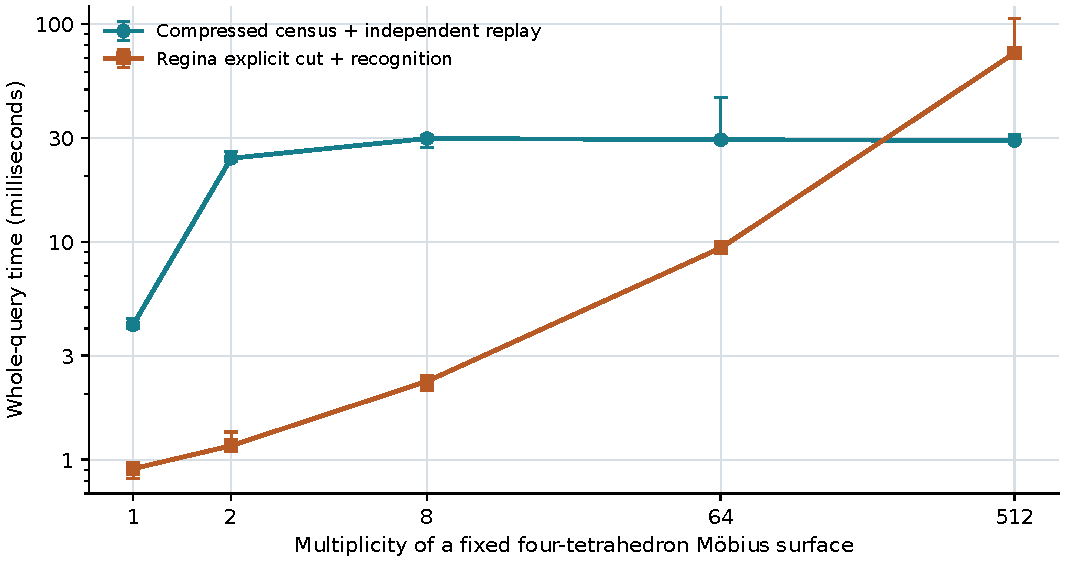
\includegraphics[width=0.94\linewidth]{figures/mobius_capacity.pdf}
\caption{Whole-cut production and verification versus explicit cut and
recognition, on one fixed source with increasing M\"obius multiplicity.
Points are seven-round medians; bars show the observed minimum and maximum.
Both axes are logarithmic. Connecting lines only guide the eye.}
\label{fig:capacity-times}
\end{figure}

On a source with three-handles, the disabled path returns early and does
not do comparable successful work. Its shorter runtime is an abstention
cost and is not used to claim a speedup or slowdown. On the three controls
without three-handles, all three strategies take the identical native
path. Their measured differences are timing variation, not forest work.
The final patch changes the default keyword from BFS to maximum weight
after these measurements; every measured call supplied an explicit
strategy, so that default change does not change the measured operation.

\subsection{Binary capacity and certificate size}

The separate capacity run multiplies the four-tetrahedron M\"obius vector
by $2^{16384}$. Both native strategies certify and independently replay
the exact census
\[
 \left(2^{16383}+1\right)H_1.
\]
The recorded single-run production-plus-replay totals are 0.1003 seconds
for BFS and 0.1088 seconds for maximum weight. Each serialized full
certificate is 5,429,503 bytes. No explicit cut of this input was attempted,
and there is no paired speedup comparison for it.

The full certificate includes the original source and orbit certificates,
which repeat some large integers. Its megabyte size must not be confused
with the added top-forest trace, whose combinatorial size is independent
of the multiplier. The test establishes that this family is handled
without one record per normal disc or component. It does not establish
optimal certificate encoding or the same time for every input of comparable
coordinate bit length. The multiplier itself has 16,385 bits.
An additional integration test cuts the five-tetrahedron loop source by
$2^{16384}$ boundary-link discs and replays the exact census
$2^{16384}H_0\sqcup H_1$.

\subsection{Regression, hostile replay, and exact algebra}

The full integrated native regression suite passes: 1,696 tests in
377.446 seconds, with no failures or errors. This includes the 12 new
dual-forest test methods and six new integration methods. The run used
the pinned repository's historical fixtures and dependent research
directories, not an incomplete extraction of the runtime folder. Its
complete log is included in \code{research/data/native\_regression.log}.


The focused native tests cover repeated interior vertices, both occurrences
of a loop, positive-weight loop splitting, reversed dependent orders,
alternative valid trees, tetrahedron and local-vertex relabelling,
source tampering, forbidden Boolean identifiers, the integer codec,
operation allowances, callback propagation, and scalar-certificate reuse.
The weighted graph producer is checked against every spanning tree on
128 small multigraph instances. Integration tests disable the relevant
producer entry points during complete v6 replay and reject wrapper removal,
nested wrappers, altered source geometry, and mismatched coordinates.

The quotient component has 27 passing tests. These include 400 deterministic
random algebraic instances, 250 independent SymPy rank comparisons, all
32 combinations of zero/nonzero chain dimensions, rational support with
a nonunit denominator, an outside witness with nonunit evaluation,
commuting-square failures, malformed matrices, stale input binding,
hostile witness mutations, and command-line round trips. The additional
16,384-bit subprocess test checks the documented large-decimal launch
configuration. These are checks of the exact algebraic contract, not
geometric examples of the future hierarchy interface.

\section{From local improvements to a global complexity theorem}
\label{sec:global}

\subsection{A complete cost ledger}

The distinction between normal weight and its encoding is essential but
insufficient. For a hierarchy state $H_i$, let $s_i$ be the full encoded
state size: source charts, current pattern, bundle identifications,
coordinate bits, and all live compressed-word or interval descriptions.
Let $a_i$ count candidate transitions that are generated, including later
discarded candidates. A useful global accounting identity has the form
\[
 T(n)\le T_{\rm input}(n)+
 \sum_{i\in\mathcal V}
 \left(T_{\rm state}(s_i)+
       \sum_{j=1}^{a_i}T_{\rm transition}(s_i,j)\right),
\]
where $\mathcal V$ contains every visited search state, including failed
branches. A polynomial bound on one summand does not control either
$|\mathcal V|$ or the maximum $s_i$.

The orbit-compression framework of Agol--Hass--Thurston supplies the right
kind of primitive for avoiding expansion in multiplicity
\cite{aht2006}. Lackenby's surface-curve algorithms likewise illustrate
operations charged to triangulation size and logarithmic curve weights
\cite{lackenby-curves}. The missing global work is to prove that the
particular hierarchy's interfaces stay within those input-size regimes
and that sufficiently few states and candidates are inspected. An
exponential number of short compressed objects is still too many objects.

\begin{proposition}[A sufficient search-tree accounting theorem]
\label{prop:global-ledger}
Suppose a deterministic recognition procedure on an $n$-crossing input
satisfies all of the following for some constants $a,b,c$:
\begin{enumerate}
\item The input conversion takes polynomial time.
\item Every visited state and every required transition certificate has
encoded size at most $n^a$.
\item At most $n^b$ children are generated at any state, and all local work
per child and per state is at most $n^c$.
\item Every root-to-leaf path in the actual explored tree has length at
most $d(n)$.
\item The branching rule is complete, the leaf predicates are sound, and
their combination correctly decides both knot answers.
\end{enumerate}
Then the total running time is $n^{O(d(n)+1)}$. In particular,
$d(n)=O(\log n)$ gives $n^{O(\log n)}$, while
$d(n)=O((\log n)^2)$ gives $2^{O((\log n)^3)}$.
\end{proposition}

\begin{proof}
The number of nodes is at most
$1+n^b+\cdots+(n^b)^{d(n)}$. Multiplying by a polynomial upper bound on
local work, including child generation and verification, gives the stated
bound. The final assertions follow by substituting the two depth estimates
and taking logarithms. The correctness hypothesis is listed separately
because a fast incomplete search would not prove a recognition theorem.
\end{proof}

The proposition is an accounting tool, not a claim that the hypotheses
already hold. In particular, it cannot be applied with the depth of one
successful path when the algorithm may search much deeper failed paths.
Memoization can improve this bound only after an authenticated equivalence
relation on states and a bound on distinct reachable equivalence classes
are proved.

\subsection{Strict quadratic decrease is weaker than multiplicative decrease}

Write $q=c_q(H)$ for Lackenby's quadratic complexity. The homological
certificate gives a strict raw drop of at least two under its stated
hypotheses. Along a retained forward chain whose other operations are
independently $q$-nonincreasing, there can therefore be at most
$\lfloor q_0/2\rfloor$ such strict cuts. This bound is useful: it excludes
indefinite repetition of these progress steps. It is generally linear in
the initial potential and gives neither logarithmic depth nor a bound on
the number of discarded attempts.

An attempted proof must also distinguish no progress from no available
certificate. The homology quotient may vanish, or a candidate may lie
inside the bundle image, while a geometric cut still lowers $q$. Conversely,
a nonzero quotient does not itself produce an admissible, efficiently
encoded connected normal surface. The quotient test supplies a sufficient
progress predicate after geometry has been authenticated.

There is a precise stronger target for a surface constructor. For a raw
cut, write $I_H\ge0$ for each parent zero-handle's integral index and
$i_{Ha}\ge0$ for the indices of all its children, so that
$\sum_a i_{Ha}=I_H$. Then $q=\sum_H I_H^2$.

\begin{proposition}[Balanced index splitting forces multiplicative progress]
\label{prop:balanced-index}
Suppose $q>0$. Let $0<\alpha\le1$ and $0<\delta<1$. Assume that a set
$\mathcal U$ of parent zero-handles satisfies
\[
 \sum_{H\in\mathcal U}I_H^2\ge\alpha q,
 \qquad
 \max_a i_{Ha}\le(1-\delta)I_H
 \quad(H\in\mathcal U).
\]
Then
\[
 q(H\cut S)\le(1-\alpha\delta)q(H).
\]
The same upper bound holds after any cleanup whose nonincrease of $q$
has been separately established.
\end{proposition}

\begin{proof}
For $H\in\mathcal U$, nonnegativity and index conservation give
\[
 \sum_a i_{Ha}^2\le (\max_a i_{Ha})\sum_a i_{Ha}
 \le(1-\delta)I_H^2.
\]
For any other parent, the same argument without the balance assumption
gives $\sum_a i_{Ha}^2\le I_H^2$. Summing proves a drop of at least
$\delta\sum_{H\in\mathcal U}I_H^2\ge\alpha\delta q$. The cleanup
assertion is immediate from its separately supplied nonincrease.
\end{proof}

For fixed positive $\alpha,\delta$, a forward nonincreasing chain can have
only $O(\log(q_0+1))$ such balance stages while its potential remains
positive. More precisely, after $k$ of them the potential is at most
$(1-\alpha\delta)^kq_0$; integrality bounds $k$ until the potential
vanishes or balance ceases to be available. This does not assert existence
of a next balance stage. An index-one parent cannot be split into
nonnegative integer children with maximum at most $(1-\delta)I_H$.
The residual small-index situation requires a separate geometric treatment,
and neutral stages and failed searches need their own bounds.

The inequality identifies the missing construction theorem more sharply
than the phrase ``find a useful surface.'' One would need to find a
compressed surface or a controlled batch that separates a fixed fraction
of the squared-index mass, or else returns a certified alternative region
whose handling admits an equally strong amortized estimate. An
outside-image witness guarantees some separation, but gives no uniform
fraction of the mass.

\subsection{A sharper raw-cut accounting potential}

The same identity gives a useful local reformulation. Define
\[
 \ell(H)=\sum_H I_H,\qquad
 P(H)=\sum_H\binom{I_H}{2}=\frac{q(H)-\ell(H)}{2}.
\]
Here $P$ counts unordered pairs of index units lying in the same parent.
This interpretation is arithmetic and does not assume those units have
canonical geometric representatives.

\begin{proposition}[Pair-separation accounting]
\label{prop:pair-potential}
For a raw normal cut satisfying nonnegative integral child indices and
per-parent index conservation,
\[
 \ell(H\cut S)=\ell(H),\qquad
 P(H)-P(H\cut S)=\sum_H\sum_{a<b}i_{Ha}i_{Hb}.
\]
Thus an outside-image cut from the progress theorem lowers $P$ by at least
one. Along a sequence consisting only of such raw cuts, the number of
strict cuts is at most $P(H_0)$.
\end{proposition}

\begin{proof}
Sum the conservation identities for the first equality. Subtract this
equality from the quadratic defect identity and divide by two for the
second. Each summand is a nonnegative integer. A positive quadratic defect
therefore gives an integral drop of at least one, and the final assertion
follows by telescoping the nonnegative potential.
\end{proof}

The qualification ``raw'' is necessary. Nonincrease of $q$ alone does not
imply nonincrease of $P$ if a subsequent operation changes $\ell$. For
example, as abstract index inventories, four indices equal to one and a
single index equal to two both have $q=4$, but their values of $P$ are zero
and one. This arithmetic example is not asserted to be an available
geometric cleanup. It shows why a proof of a cleanup rule for $q$ cannot
simply be relabelled as a proof for $P$.

The terminal condition $P=0$ means that every remaining index is zero or
one. It does not mean that the manifold is a ball, that its pattern is
essential, or that a knot is unknotted. A useful future strategy could
separate the problem of reducing index concentration from the classification
of this small-index remainder, provided both stages preserve the required
boundary data.

There is an even sharper count for a raw-only sequence. Let $r(H)$ be the
number of positive-index zero-handles. Every positive parent has at least
one positive child, every zero parent has only zero children, and a strict
raw cut has some parent with at least two positive children. Thus each
strict cut increases $r$ by at least one. Since $r\le\ell$ and $\ell$ is
conserved, the number of strict raw cuts is at most
\[
 \ell(H_0)-r(H_0)=\sum_H\max\{I_H-1,0\}\le P(H_0).
\]
The last inequality follows from $k-1\le\binom{k}{2}$ for every integer
$k\ge1$. The pair potential supplies the exact weighted defect; the
positive-child count supplies the sharper elementary number-of-cuts bound.
Neither extends through arbitrary cleanup without additional conservation
or monotonicity information.

\subsection{What the dual-forest theorem contributes to this ledger}

The top reduction resolves a specific local obstruction with polynomial
encoded work and a coordinate-magnitude-independent additional trace. It
does not add a large branching factor: the default uses one optimized tree.
Its optional complete restricted search has cost
$t^{O(v_3)}\operatorname{poly}(t,L)$ for $v_3$
interior source vertices, and hence is quasi-polynomial in the full encoded
source input when $v_3=O(\log t)$. This is a correct parameterized result for the stated
compiler family. No argument in this article makes $v_3$ logarithmic along
an arbitrary full recognition hierarchy or proves that that compiler family
is topologically complete.

Removing source three-handles also helps align a normal cut with interfaces
that require none. However, it preserves the specified bundle ports, not
an arbitrary hierarchy boundary pattern, and it does not automatically
establish Lackenby-admissibility. These remaining conditions are precisely
where a tempting informal composition would otherwise become invalid.

\section{Further research questions and concrete next investigations}
\label{sec:agenda}

The following programme is ordered by the dependencies exposed by the
proofs and experiments. Each item names a specific mathematical or software
deliverable and the evidence that would justify moving to the next step.
The questions are proposals, not claims already established by this article.

\subsection{Immediate source-compiler research}

\paragraph{1. Joint primal and dual forest selection.}
The paired-forest objective gives exact coordinate optimizations of retained
unsigned incidence. Implement it as an optional producer while keeping the
existing independent forest and cancellation checker. Measure successful
censuses, retained occurrences, total query time, and certificate size
separately. Does alternating selection ever improve certified coverage over
the current canonical-primal, maximum-dual choice on actual sources?
If it does, find a small explicit face table and a stopping-set proof of
strictness, as in the five-tetrahedron example. A mere reduction in the
objective would not answer the coverage question.

\paragraph{2. Obstruction-guided dual-tree search.}
Given a failed residual, extract its maximal stopping core. Every successful
tree must meet that core in an eligible source row. Branch only on such
edges, reject forced cycles immediately, and use the graphic-rank
obstruction to prune incompatible families. Prove that each pruning rule
preserves all successful trees. The unrestricted worst-case bound remains
$t^{O(v_3)}$; the useful question is whether source geometry bounds the
number of relevant stopping cores or supplies a smaller structural
parameter. A succinct failed-search proof would certify failure of this
compiler family, not nontriviality of a knot.

\paragraph{3. The eight surviving positive corpus obstructions.}
The explicit-cut audit identifies these current targets:
\begin{center}\small
\begin{tabular}{ll}
\texttt{pilot/fibonacci\_lst\_04/0} & \texttt{pilot/fibonacci\_lst\_06/0}\\
\texttt{pilot/fibonacci\_lst\_08/0} & \texttt{pilot/fibonacci\_lst\_10/0}\\
\texttt{pilot/lst\_4\_9/0} & \texttt{pilot/finite\_trefoil/0}\\
\texttt{pilot/finite\_figureEight/0} & \texttt{pachner23\_5\_8\_2/mixed}.
\end{tabular}
\end{center}
They were already beyond the source-three-handle refusal, so the present top
reduction alone cannot resolve them. Determine whether another primal
forest suffices; otherwise produce a geometrically authenticated
intersection-reducing move, change of disk system, or boundary normalization
that destroys the stopping core. The completeness of positive raw peeling
means that merely searching more positive pivot orders on the same matrix
cannot be the remedy. A successful next contribution should include the
smallest actual source obstruction it changes and the new geometric replay
rule it needs.

\paragraph{4. Source-realizable exchange structure.}
The abstract peelable-row system is not a matroid. Are there narrower
families of endpoint-gap source matrices with a useful exchange or bounded
obstruction property? Conversely, can the minimal three-by-two and Boolean
four-by-three counterexamples be realized, with their full row systems,
by authenticated finite normal cuts? Either result would sharpen the
algorithm-design options. No inference about geometric realizability
should be drawn from a presentation matrix alone.

\paragraph{5. Avoiding repeated source preparation and proof duplication.}
The graph trace is small, but the enclosing verifier currently reconstructs
some source data in several layers, and the largest demonstrated full
certificate exceeds five megabytes. Design an immutable authenticated
source object with explicit consumer contracts. Prove which derived facts
can be reused without trusting a producer, and measure complete replay
time and bytes. For wire-format deduplication, reference shared integer or
source blocks through checked identifiers and retain exact source binding.
The target is reduced repeated work, not a weaker authenticity check.

\subsection{Geometric realization of homological progress}

\paragraph{6. Compile the actual relative bundle inclusion.}
Construct compatible finite chain complexes for
$(\mathcal B,\mathcal B\cap\partial M)$ and $(M,\partial M)$ from an
authenticated admissible patterned handle structure. Produce and verify
the actual matrices $d_2,d_3,\delta_2,j_1,j_2$, and prove polynomial bounds
on their ranks, entries, and construction time in the maintained encoding.
The key issue is the embedded inclusion, including signs, horizontal versus
vertical boundary, twisted bundles, and any peripheral identifications.
An abstract homology computation or an unsigned incidence matrix is
insufficient. Validate the first compiler on small triangulations whose
relative chain maps can also be built independently by subdivision.

\paragraph{7. Authenticate the prescribed cohomology-class constructor.}
Build the chain-level duality map and the normal representative of a chosen
integral $H^1$ class, preserving that class through every normalization.
Retain the no-three-handle and local-type hypotheses of the handle version
of the construction. Can every intermediate operation be expressed using
the project's compressed coordinates and verified pattern charts? A useful
first theorem would give a polynomial bit bound for one complete prescribed
class construction, including the resulting signed cycle certificate.

\paragraph{8. Extract one component using a signed scalar witness.}
The component lemma suggests a smaller interface than computing a full
homology vector for every component. Given one annihilating row $Y$ and an
oriented compressed surface with positive total evaluation, find a component
with $Y$-evaluation positive and certify its actual oriented relative cycle.
Develop the signed weighted-orbit semantics and a source-authenticated
component selector. The selector must handle cancellation between positive
and negative contributions and cannot rely on unsigned counts alone.
Compare its representation size against a full vector-valued component
calculation.

\paragraph{9. Understand quotient-zero states.}
When $H_2(M,\partial M;\mathbb Q)/V_{\mathcal B}=0$, the proposed predicate
has no outside class to select. Characterize those states geometrically
under the hierarchy's actual admissibility assumptions. Do they admit a
bounded collection of bundle-supported moves, a certified product-region
description, or a different decreasing invariant? The task is an
alternative construction theorem; absence of an outside witness is not
a terminal recognition criterion.

\paragraph{10. Simultaneous cuts and changing bundle images.}
For disjoint oriented surfaces $S_1,\ldots,S_k$, study the rank of their
classes modulo the initial bundle image and its relation to the raw
quadratic defect of the simultaneous cut. Is there a lower bound such as
twice that rank under appropriate hypotheses, or a small genuine
counterexample? The one-surface theorem does not prove such a statement:
the actual interior parallelity bundle changes after a cut, so sequential
quotients cannot silently be identified. A solution needs compatible
relative maps and a theorem controlling their change.

\subsection{The global quantitative problem}

\paragraph{11. Construct balanced cuts or certified alternatives.}
Proposition~\ref{prop:balanced-index} gives a concrete sufficient condition
for multiplicative quadratic progress. Can one find a surface or a
controlled batch that splits a constant fraction of the squared-index
mass, or else identify a geometrically structured region with a different
amortized simplification rule? In particular, analyze the obstruction from
index-zero and index-one pieces instead of assuming balance continues
indefinitely. The intended result must include a construction cost and
compressed output-size bound, not only existence of a balanced surface.

\paragraph{12. Transport a full boundary pattern through top cancellation.}
The present theorem is relative to the actual bundle ports. A future
hierarchy may carry marks across the exposed faces of selected endpoint
gaps. Design an explicit map of those curves and arcs through the
cancellation neighbourhood, including corner rounding, order, orientation,
and component ownership. Prove bounds on the resulting compressed word
size and geometric intersection complexity. Is there a forest objective
that minimizes this transport cost as well as raw attaching incidence?
Without such a theorem, using the native top reduction as an arbitrary
patterned hierarchy move would exceed its proved interface.

\paragraph{13. Count discarded histories and rebuilding work.}
State the exact search algorithm and assign an amortized charge to every
candidate, failed surface, restored pattern, and rebuilt source chart.
Can a multisurface batch retain enough geometric and homological information
to avoid reconstructing a long prefix after one branch fails? The desired
bound must apply to all visited histories. A logarithmic bound on one
retained successful chain and a polynomial-size certificate for that chain
are not enough.

\paragraph{14. Bound the complete maintained representation.}
Prove polynomial bounds in the original crossing number for every live
chart count, compressed word grammar, interval-family list, relative chain
rank, matrix entry, and coordinate bit length. Then verify that every
consumer is polynomial in that \emph{same} representation. Local type
bounds alone do not limit the number of repeated local pieces, and binary
encoding alone does not limit the number of distinct binary records.
This accounting should be machine-readable enough that experiments can
log every parameter appearing in the theorem.

\paragraph{15. Formulate and prove the exact final asymptotic statement.}
Choose whether the theorem targets $n^{O(\log n)}$ or the weaker
$2^{O((\log n)^3)}$ formulation, and specify all hypotheses, input
conversions, arithmetic conventions, and constants hidden by the notation.
Establish completeness on arbitrary knot diagrams and correctness of both
answers. Only then combine the encoded-state, branching, and explored-depth
bounds using Proposition~\ref{prop:global-ledger}. The local results in this
article provide useful components for that proof, but do not replace it.

\subsection{Recommended order of work}

The most direct engineering continuation is the joint-forest producer and
the eight positive stopping obstructions, with the existing checker kept
as the acceptance boundary. In parallel, the most consequential new
geometric interface is the authenticated relative chain map, followed by
the signed component selector. Those steps make the homological predicate
available to real hierarchy states. Balanced construction, pattern
transport, and a charge for discarded histories are then the central
mathematical obstacles to the global bound. This order keeps empirical
coverage gains connected to explicit lemmas and avoids treating a collection
of fast local routines as an already complete recognition algorithm.

\appendix
\section{Artifact contents and reproduction}
\label{app:reproduction}

The accompanying archive contains the complete \LaTeX{} source, bibliography,
vector and raster figures, compiled article, integration patch, source
overlay, a compact frozen runtime, independent algebraic code, source
fixtures, saved certificates, raw experimental records, and validation
logs. The top-level \code{README.md} is the practical entry point.
\code{SHA256SUMS} authenticates the packaged files against accidental
changes; \code{provenance/source\_pin.json} records the baseline revision
and workload identifiers.

\begin{table}[htbp]
\centering
\begin{tabular}{P{0.31\linewidth}P{0.62\linewidth}}
\toprule
Path & Purpose\\
\midrule
\code{article/} & Main TeX file, included sections, bibliography, figures,
and the compiled PDF.\\
\code{integration/} & Patch against the pinned ProveIt revision and an
equivalent nine-file source overlay. Apply one method, not both.\\
\code{runtime/fast/} & Frozen runtime and focused fixtures/tests for
standalone reproduction of this contribution. It is not a replacement
for the full repository and its historical regression data.\\
\code{research/experiments/} & Corpus audit, explicit Regina oracle,
paired timings, exact matrix witness, figure generation, and summary
scripts.\\
\code{research/data/} & Original 106-case workload; baseline, BFS,
weighted, and explicit-cut JSON; paired timing samples; test logs and
machine-readable summaries.\\
\code{research/certificates/} & Saved source-bound census certificates,
including all seven newly completed maintained cases under both trees.\\
\code{research/quotient/} & Standalone exact chain-pair producer,
independent verifier, examples, tests, and interface documentation.\\
\code{provenance/} & Pinned tree manifests, source identifiers, artifact
claim ledger, and integration validation.\\
\bottomrule
\end{tabular}
\end{table}

\subsection{Build and focused checks}

From the extracted archive, the principal commands are:
\begin{lstlisting}[language=bash]
python reproduce.py --quick
cd article
latexmk -pdf -interaction=nonstopmode -halt-on-error \
  dual_forests_and_homological_progress.tex
\end{lstlisting}
The quick command checks packaged hashes, runs the 18 focused native test
methods and 27 algebraic test methods, and replays saved census packets.
It uses Python's standard library for native production and verification;
SymPy enables the additional independent algebraic rank comparison.
Regina is required only for explicit-cut audits and the paired timing
script. The figure script uses Matplotlib. Full command details and the
recorded environment are in the README.

The main corpus can be rerun using the frozen runtime with
\code{PYTHONPATH=runtime/fast} and
\code{research/experiments/audit\_native.py}; explicit comparisons use
\code{audit\_regina.py}. The baseline audit was run on the untouched
pinned implementation. It can be regenerated in a checkout of that
revision, while the delivered \code{disabled} mode reproduces its
three-handle refusal for diagnostic comparisons. The paired benchmark
supplies every strategy explicitly and records its code hashes.

\subsection{Repository integration}

Apply \code{integration/dual\_forest.patch} in a complete ProveIt checkout
at the pinned revision. It adds the two runtime modules,
two focused test modules, three source/experiment helpers, and modifies
the producer and independent verifier of the normal-cut handlebody census.
The patch adds no third-party dependency to native recognition.

The full regression command, run from
\code{Topology/UnknotRecognition/fast}, is
\begin{lstlisting}[language=bash]
python -m unittest discover -s tests -v
\end{lstlisting}
Some existing tests require the repository's \code{reports/} and
\code{synthesis/} data and an older Git source object. Those dependencies
are part of the full project, rather than duplicated into this focused
archive. The archived successful run used them. A reduced runtime-only
extraction should use the quick focused checks instead of treating missing
historical research files as algorithm failures.

The integration validation checks that the patch applies to the exact
baseline and produces the same changed files as the supplied overlay.
The article and algebraic research component can be placed in the repository's
preferred incoming or proposal directory independently of applying the
runtime patch.

\subsection{Independent review and reproducibility limits}

The source-relative theorem, loop multiplicities, relative-port statement,
native strict example, and v6 integration were reviewed separately from
their producer implementation. The homology alternative, duality degrees,
chain-map hypotheses, exact defect, and global accounting statements also
received a separate mathematical review. These reviews motivated explicit
limits in the final text, particularly the raw/cleanup distinction,
arbitrary-pattern transport, and the difference between an additive
potential drop and a global search bound.

This is a research contribution supplied for further mathematical and code
review. Its executable verifiers, exact examples, proofs, and logs make
specific claims inspectable. They are not evidence that the unimplemented
geometric interfaces already exist, and the selected timing family cannot
establish a universal asymptotic complexity class.

\section{Claim ledger}
\label{app:claims}

The following ledger records the logical status of the main statements.
``Proved'' refers to the mathematical statement in the cited section;
``implemented'' refers to the specific delivered code and contract.

\begin{longtable}{P{0.27\linewidth}P{0.24\linewidth}P{0.40\linewidth}}
\toprule
Claim & Status & Scope and evidence\\
\midrule
\endhead
Ordinary empty-pattern source two/three cancellation & Prior repository
result & Credited to the incoming genus-budget contribution; not asserted
as new here.\\
Complete cut-relative source top reduction & Proved and implemented &
Theorem~\ref{thm:cut-dual-complete}; authenticated source normal cuts,
including empty and one-sided surfaces; relative to actual bundle ports.\\
Top trace independent of normal magnitudes & Proved and tested &
Proposition~\ref{prop:cut-dual-cost}; original source validation still
depends on coordinate bits.\\
Same-zero-support trace reuse & Proved; tests included &
Proposition~\ref{prop:cut-dual-support}; requires source reauthentication;
arbitrary same-support costs need not remain optimal.\\
Minimum retained additive cost & Proved and implemented &
Theorem~\ref{thm:cut-dual-weighted}; fixed primal forest and fixed additive
row costs; no general recognition optimum.\\
Strict native forest-choice advantage & Proved, implemented, explicit-cut
checked & Proposition~\ref{prop:cut-dual-native-strict}; complete
five-tetrahedron source data and a persistent stopping obstruction.\\
Raw stopping-set completeness & Prior repository result & Used to
characterize the effect of a changed top forest; not a new peeling theorem.\\
Tree-transversal and rank obstruction & Proved consequences &
Theorem~\ref{thm:cut-dual-stopping} and
Corollary~\ref{cor:cut-dual-rank-obstruction}; failure is restricted to
this compiler family.\\
Peelable-row matroid exchange & Refuted in general &
Proposition~\ref{prop:cut-dual-nonmatroid}; minimal and Boolean abstract
counterexamples; no unsupported source realization.\\
Restricted exhaustive forest search & Proved; not added to the default &
Proposition~\ref{prop:cut-dual-search}; $t^{O(v_3)}\operatorname{poly}(t,L)$
for polynomial-size source incidence.\\
Alternating paired-forest optimization & Proved proposal; unimplemented &
Proposition~\ref{prop:paired-forests}; polynomial for literal bounded source
incidence; conditional minima need not be joint minima.\\
Rational bundle-image certificate alternative & Proved and implemented
algebraically & Theorem~\ref{thm:quotient-alternative}; integer replay and
polynomial witness bounds; geometry is an additional contract.\\
Outside-image strict progress & Proved corollary with explicit hypotheses &
Theorem~\ref{thm:quotient-strict-progress}; actual admissible hierarchy and
interior bundle required; exact formula before cleanup.\\
Reuse of a separating row for one component & Proved &
Lemma~\ref{lem:quotient-component}; oriented signed component data,
new evaluation and input binding required.\\
Polynomial geometric progress constructor & Conditional interface &
Proposition~\ref{prop:quotient-interface}; source chain compiler,
prescribed-class normalization, and signed component extraction remain open.\\
Balanced multiplicative potential decrease & Proved sufficient criterion &
Proposition~\ref{prop:balanced-index}; no existence claim for a balanced
cut, no bound on neutral or discarded work.\\
Pair-separation potential and positive-child count & Proved raw-cut
identities/bounds & Proposition~\ref{prop:pair-potential} and following
argument; arbitrary cleanup needs additional hypotheses.\\
85 to 92 maintained-corpus successes & Reproduced experiment &
Unchanged pinned 106-case corpus; all old successes preserved, positive
certificates independently replayed.\\
No false positive in explicit comparisons & Reproduced experiment &
85 directly comparable native positives agree; 99 explicit computations
complete; seven large cases outside expansion cap.\\
Native binary-capacity result & Reproduced single workload &
$2^{16384}$ scaling; exact $2^{16383}+1$-component census; capacity, not an
asymptotic fit.\\
Full quasi-polynomial unknot recognition & Not proved by this contribution &
Global encoded-size, construction, completeness, branching, explored-depth,
and pattern-transport obligations remain in Section~\ref{sec:agenda}.\\
\bottomrule
\end{longtable}

\bibliographystyle{plain}
{\raggedright\bibliography{references}}
\end{document}
